\documentclass[11pt,twoside]{article}

\usepackage{forest}
\usepackage{graphicx}
\usepackage{wasysym}
\usepackage{url}


\usepackage[backend=biber,style=alphabetic]{biblatex} 
\addbibresource{ref.bib}  


%%%%%%%%%%%%%%%%%%%%%%%%%%%%%%%%%%%%%%%%%%%%%%%%%%%%%%%%%%%%%%%%%%%%%%%%%%%%%

% Definitions for the title page
% Edit these to provide the correct information
% e.g. \newcommand{\reportauthor}{Timothy Kimber}

\newcommand{\reporttitle}{A digital interface designed for sharing diagnostic medical imaging with patients}
\newcommand{\reportauthor}{Laura Hagege LH}
\newcommand{\supervisor}{Fernando Bello}
\newcommand{\degreetype}{Msc Computing Science}

%%%%%%%%%%%%%%%%%%%%%%%%%%%%%%%%%%%%%%%%%%%%%%%%%%%%%%%%%%%%%%%%%%%%%%%%%%%%%

% load some definitions and default packages
%%%%%%%%%%%%%%%%%%%%%%%%%%%%%%%%%%%%%%%%%
% University Assignment Title Page 
% LaTeX Template
% Version 1.0 (27/12/12)
%
% This template has been downloaded from:
% http://www.LaTeXTemplates.com
%
% Original author:
% WikiBooks (http://en.wikibooks.org/wiki/LaTeX/Title_Creation)
%
% License:
% CC BY-NC-SA 3.0 (http://creativecommons.org/licenses/by-nc-sa/3.0/)
% 
%
%%%%%%%%%%%%%%%%%%%%%%%%%%%%%%%%%%%%%%%%%
%----------------------------------------------------------------------------------------
%	PACKAGES AND OTHER DOCUMENT CONFIGURATIONS
%----------------------------------------------------------------------------------------
\usepackage[a4paper,hmargin=2.8cm,vmargin=2.0cm,includeheadfoot]{geometry}
\usepackage{textpos}
\usepackage{natbib} % for bibliography
\usepackage{tabularx,longtable,multirow,subfigure,caption}%hangcaption
\usepackage{fncylab} %formatting of labels
\usepackage{fancyhdr} % page layout
\usepackage{url} % URLs
\usepackage[english]{babel}
\usepackage{amsmath}
\usepackage{graphicx}
\usepackage{dsfont}
\usepackage{epstopdf} % automatically replace .eps with .pdf in graphics
\usepackage{backref} % needed for citations
\usepackage{array}
\usepackage{latexsym}
\usepackage[pdftex,pagebackref,hypertexnames=false,colorlinks]{hyperref} % provide links in pdf

\hypersetup{pdftitle={},
  pdfsubject={}, 
  pdfauthor={},
  pdfkeywords={}, 
  pdfstartview=FitH,
  pdfpagemode={UseOutlines},% None, FullScreen, UseOutlines
  bookmarksnumbered=true, bookmarksopen=true, colorlinks,
    citecolor=black,%
    filecolor=black,%
    linkcolor=black,%
    urlcolor=black}

\usepackage[all]{hypcap}


%\usepackage{color}
%\usepackage[tight,ugly]{units}
%\usepackage{float}
%\usepackage{tcolorbox}
%\usepackage[colorinlistoftodos]{todonotes}
% \usepackage{ntheorem}
% \theoremstyle{break}
% \newtheorem{lemma}{Lemma}
% \newtheorem{theorem}{Theorem}
% \newtheorem{remark}{Remark}
% \newtheorem{definition}{Definition}
% \newtheorem{proof}{Proof}


%%% Default fonts
\renewcommand*{\rmdefault}{bch}
\renewcommand*{\ttdefault}{cmtt}



%%% Default settings (page layout)
\setlength{\parindent}{0em}  % indentation of paragraph

\setlength{\headheight}{14.5pt}
\pagestyle{fancy}
\renewcommand{\chaptermark}[1]{\markboth{\chaptername\ \thechapter.\ #1}{}} 

\fancyfoot[ER,OL]{\sffamily\textbf{\thepage}}%Page no. in the left on odd pages and on right on even pages
\fancyfoot[OC,EC]{\sffamily }
\renewcommand{\headrulewidth}{0.1pt}
\renewcommand{\footrulewidth}{0.1pt}
\captionsetup{margin=10pt,font=small,labelfont=bf}


%--- chapter heading

\def\@makechapterhead#1{%
  \vspace*{10\p@}%
  {\parindent \z@ \raggedright \sffamily
    \interlinepenalty\@M
    \Huge\bfseries \thechapter \space\space #1\par\nobreak
    \vskip 30\p@
  }}

%---chapter heading for \chapter*  
\def\@makeschapterhead#1{%
  \vspace*{10\p@}%
  {\parindent \z@ \raggedright
    \sffamily
    \interlinepenalty\@M
    \Huge \bfseries  #1\par\nobreak
    \vskip 30\p@
  }}

\allowdisplaybreaks

% load some macros
% Here, you can define your own macros. Some examples are given below.

\newcommand{\R}[0]{\mathds{R}} % real numbers
\newcommand{\Z}[0]{\mathds{Z}} % integers
\newcommand{\N}[0]{\mathds{N}} % natural numbers
\newcommand{\C}[0]{\mathds{C}} % complex numbers
\renewcommand{\vec}[1]{{\boldsymbol{{#1}}}} % vector
\newcommand{\mat}[1]{{\boldsymbol{{#1}}}} % matrix


\date{September 2018}

\begin{document}

% load title page
% Last modification: 2015-08-17 (Marc Deisenroth)
\begin{titlepage}

\newcommand{\HRule}{\rule{\linewidth}{0.5mm}} % Defines a new command for the horizontal lines, change thickness here


%----------------------------------------------------------------------------------------
%	LOGO SECTION
%----------------------------------------------------------------------------------------


\includegraphics[width = 4cm]{./figures/imperial}\\[0.5cm] 

\center % Center remainder of the page

%----------------------------------------------------------------------------------------
%	HEADING SECTIONS
%----------------------------------------------------------------------------------------

\textsc{\Large Imperial College London}\\[0.5cm] 
\textsc{\large Department of Computing}\\[0.5cm] 

%----------------------------------------------------------------------------------------
%	TITLE SECTION
%----------------------------------------------------------------------------------------

\HRule \\[0.4cm]
{ \huge \bfseries \reporttitle}\\ % Title of your document
\HRule \\[1.0cm]

%----------------------------------------------------------------------------------------
%	SUB TITLE SECTION
%----------------------------------------------------------------------------------------

\textsc{\large --- Background and Progress Report ---}\\[0.5cm] 
 
%----------------------------------------------------------------------------------------
%	AUTHOR SECTION
%----------------------------------------------------------------------------------------



\emph{by} \\
\reportauthor % Your name

~

\emph{Supervisor:} 
\supervisor % Supervisor's Name




%----------------------------------------------------------------------------------------
%	FOOTER & DATE SECTION
%----------------------------------------------------------------------------------------
\vfill % Fill the rest of the page with whitespace
Submitted in partial fulfillment of the requirements for the MSc degree in
\degreetype~of Imperial College London\\[0.5cm]

\makeatletter
\@date 
\makeatother


\end{titlepage}



% page numbering etc.
%\pagenumbering{roman}
%\clearpage{\pagestyle{empty}\cleardoublepage}
%\setcounter{page}{1}
%\pagestyle{fancy}

%%%%%%%%%%%%%%%%%%%%%%%%%%%%%%%%%%%%
%\begin{abstract}
%Your abstract.
%\end{abstract}

%\cleardoublepage
%%%%%%%%%%%%%%%%%%%%%%%%%%%%%%%%%%%%
%\section*{Acknowledgments}
%Comment this out if not needed.

\clearpage{\pagestyle{empty}\cleardoublepage}

%%%%%%%%%%%%%%%%%%%%%%%%%%%%%%%%%%%%
\begin{abstract}
\normalsize



"The abstract is a very brief summary of the report's contents. It should be about half page long. Somebody unfamiliar with your project should have a good idea of what it is about having read the abstract alone and will know whether it will be of interest to them."

\end{abstract}
\cleardoublepage


%%%%%%%%%%%%%%%%%%%%%%%%%%%%%%%%%%%%
\renewcommand{\abstractname}{Acknowledgements}
\begin{abstract}

"It is usual to thank those individuals who have provided particularly useful assistance, technical or otherwise, during your project. Your supervisor will obviously be pleased to be acknowledged as they will have invested quite a lot of time overseeing your progress."

Person to thank:
\newline \vspace{5mm}
- I would like to express my deep gratitude to Professor Dr Fernando Bello
\newline \vspace{5mm}
- Will Cox
\newline \vspace{5mm}
- Co-workers at Chelsea and westminster hospital
\newline \vspace{5mm}
- Developper community over the internet and around me 
\newline \vspace{5mm}



\end{abstract}
\cleardoublepage


%%%%%%%%%%%%%%%%%%%%%%%%%%%%%%%%%%%%
%--- table of contents
%\fancyhead[RE,LO]{\sffamily {Table of Contents}}
\tableofcontents 

\clearpage{\pagestyle{empty}\cleardoublepage}
\pagenumbering{arabic}
\setcounter{page}{1}
\fancyhead[LE,RO]{\slshape \rightmark}
\fancyhead[LO,RE]{\slshape \leftmark}


%%%%%%%%%%%%%%%%%%%%%%%%%%%%%%%%%%%%
\section{Introduction}

According to a study published in January 2018 from \textbf{National Health Service (NHS) England} [2], 41.4 million \textbf{imaging tests} have been reported in England between October 2016 and December 2017. Indeed, \textbf{medical imaging} exams are routinely used all over the world to explore internal body structures and/or diagnose diseases. This generic term encompasses various clinical imaging techniques, such as, \textbf{Magnetic Resonance Imaging} (MRI), \textbf{Computerized Tomography} (CT-Scan) or \textbf{X-Ray}, which produce a 2D or 3D representation of physical internal structures. 

\newline \vspace{5mm}

Methods used for those exams are common, and since the introduction of the \textbf{DICOM standard} in 1985 [3], so is the professional storage and communication system. However, when it comes to sharing diagnoses with patient, each country has developed its own methods. In the \textbf{United Kingdom}, it is uncommon that a patient gets, or even requests, access to its medical data. On demand, and providing payment, one can get his data, but, generally, patients have only access to their clinical report, by means of a general practitioner, and the medical images, themselves are never seen by the patient. 

\newline \vspace{5mm}

Simultaneously, with the evolution of technology continually improving access to data; access to \textbf{medical information}, including imaging data, has become more commonplace . However, the issue about sharing those sensitive data, is not only to promote access, but essentially to make those images understandable for non clinicians. Research has already been undertaken in the United States concerning the creation of a \textbf{``patient portal"} [4] - fully designed to facilitate \textbf{patient understanding} - exploring the related opportunities, and scaling different levels of benefit. 

\newline \vspace{5mm}

Considering those facts, \textbf{Dr Fernando Bello} and \textbf{Pr William Cox} have decided to deepen the subject of designing a \textbf{patient portal}. First, by exploring the \textbf{benefits and risks} of sharing medical information with patients, and thereafter by effectively building such an interface. Consequently, after a year of background researches, they offered to work on the creation of \textbf{``A digital interface designed for sharing diagnostic medical imaging with patients"}, as a final personal project to the \textbf{department of Computing Science at Imperial College of London}, together with the \textbf{Chelsea and Westminster Hospital}. Aiming to build an interface \textbf{suitably made for imaging patients} in order to let them access and understand their medical results in the most significant and comprehensible way.

\newline \vspace{5mm}
The following report contains an overview of the work undertaken during almost three month beginning mid May 2018 under the supervision of \textbf{Dr Fernando Bello} and \textbf{Pr William Cox}. The following sections will develop in a logical order - for better understanding - the several steps reached during the conception of the interface, including issues, skills earned and personal review. 

\newline \vspace{5mm}
//Introduce the plan - will do once it is certain

  


 







\clearpage



%%%%%%%%%%%%%%%%%%%%%%%%%%%%%%%%%%%%
\section{Background and Related Work}
\textbf{DICOM standard} is a special software integrated format dedicated to \textbf{ease data storage and communication} between different facilities in the \textbf{medical imaging field}. This standard has been defined by the \textbf{American College of Radiology} (ACR) and the \textbf{National Electrical Manufactural Association} (NEMA) in 1985. DICOM defines a specific data model structure, a file format and data dictionary, it also comes with a TCP/IP protocol to facilitate data transfer. Before the creation of this standard, it was challenging for distinct services to exchange imaging information, currently DICOM format is widely use among the medical imaging area. 

\newline \vspace{5mm}
DICOM standard is a well-structured but also hard to reach software. Even if its website [7] provides a wide documentation, it remains challenging to fully understand it. The aim of the following subsection is to give a basic overview of DICOM standard structures. In the scope of my project I will mainly focus on the data storage and treatment, TCP/IP protocol has not been part of my concern. Moreover, as complete the DICOM standard website could be, I used several websites [8] \& [9], to build my understanding on the DICOM file format. 




\subsection{Project context}
%will work and goal
--> Will PhD work 
\newline
--> litterature review
\newline
--> developp section about benefit



Providing medical data to a patient is always a delicate step in a medical procedure. According to medical imaging, there are 2 manners to share data with patient, either under the control of a clinical expert, or recently via standalone technologies which could left the patient with some doubts.  

While sharing this data on a digital interface > benefit tot. discuss
Subject of will pHD, define in its report + litterature review, a lot of article 

Before beginig to work --> read though those paper and understand the challenges of this project and why 


Challenges to create an interface that could be sufficiant or provide enough to guide on the right track



PATIENT PORTAL = view medical report online 
PORTAL CAN BE "DYNAMIC AND TAILORED to patient information preference"  IPAD 2

creating an interface that can be progressively adapted in order to fit patient needs.

Why the project: 

Medical Imaging exams are routinely used to explore the human body and detect disease. 

In the litterature: experience and perceive patient needs in terms of information sharing 
--> IPAD2 = making a study on the benefit of sharing information with patient, how to share, what to share, how will patients reacts - focusedd on lung cancer patient (Los angeles)

A LOOOOOt of litterature in this field, a lot of background work on the benefit, my work come as the final stage of this question

2 BENEFIT: related and unrelated (education etc)

WILL PHD --> explore/ quantify the benefit --> MY WORK: SET UP his work in order to test it 

Some sample patient portal already done 

There are plenty of interface to deal with medical imaging but they are all made for doctors. 


With this project we want to make something accessible for the patient and valuable for them --> will levels of benefit 


With concern to provide patient with some "right" information and don't let them look over the internet for wrong answers
-> examples and talking with doctors



\clearpage
\subsection{Related Work}
Before we started to actually discuss the project goal, Will provided me with several documents, either literature reviews or articles already referenced above, concerning works and researches directly related to the project. Among those, he also provided me with the late stage report of his PhD, containing the state of play of his work at that stage. Those papers have allowed me to understand the background of the project and to identify the related issues and challenges. 

\newline \vspace{5mm}
The goal of Will's PhD is to identify the \textbf{risks and benefits} related to the creation of a patient-oriented interface. To be more precise I would cite directly from this report:

\newline \vspace{5mm}

\textit{``Intuitively, there are benefits available from sharing images with patients. Indeed, there is a wealth of research available which assesses how visualisation aids increased understanding, or promotes communication. However, little research assesses the value of radiological images in this context. Moreover, no work assesses the risks associated with sharing patients’ images with them. This is the gap which this PhD will address. The research questions for this PhD are, therefore:
\begin{itemize}
	\item Is there additional benefit that can be extracted from diagnostic images?
	\item If so, what are the requirements to enable the realisation of this benefit?"
\end{itemize}}

\newline \vspace{5mm}
Specifically, to lead his researche, he has divided benefits in two categories:
\textit{
\begin{itemize}
	\item ``Primary benefits – benefits related to the rationale for acquiring the image, e.g. diagnosis, assessment, interventional guidance
	\item Secondary benefits – benefits unrelated to the rationale for acquiring the image, e.g. education, communication, empowerment"
\end{itemize}
}

\newline \vspace{5mm}
At the moment, Will has achieved a significant work, he has completed a literature review, to set up the background and understand the issues related to the creation of a patient portal. Precisely, the aim was ``to ensure that this was a suitable subject for research and to identify any pertinent gaps in the existing knowledge.".  He also carried out a survey, questioning medical experts, supplemented with 8 semi-structured interviews in order identify and scale the related risks and benefits from a clinician point of view. the results of those works are available for consultation on \textbf{\textit{Appendix 1}. In the future the objective is to interview patients, on the same model as clinicians, to evaluate the non-clinician opinion.
  













\clearpage
\subsection{Goal definition}
Once familiar with the project background, it has been easier for me to understand the main \textbf{issues and challenges} and to have a precise idea of the goal to achieve. The objective of this project is not to simply copy and create another standard DICOM viewer but to create an interface that can be \textbf{progressively adapted to fit patient needs}. Challenges consist in buildging an interface that could be sufficient and valuable, meaning it could provide enough information to guide the patient on the right track without any simultaneous external contribution. Moreover, designing this interface should allow to identify the benefit to be realised through providing people with their imaging data, whilst also minimising the identified risks of this process.

\newline \vspace{5mm}
It has been agreed that we would together with Fernando and William, define project specifications (in terms of design and content) and that all information relative to benefits and content would be discussed mainly with William. They, also advised me to install some already existing DICOM viewer made for clinicians. They wanted me to get an idea of the kind of interface that I could produce, while keeping in mind that the goal is not to create a copy of those readers, but to produce my own patient-oriented interface.

\newline \vspace{5mm}
In the following part, I will develop the project specifications that have been produced in the early stage of the project, following multiple discussion with my tutors. Moreover, considering that I have been given complete freedom in the choice of the tools and languages to use for building the interface, I will explain the choices I have made before starting to implement my project.






\clearpage
%%%%%%%%%%%%%%%%%%%%%%%%%%%%%%%%%%%%
\section{Early Specifications and Implementation Methods}
\textbf{DICOM standard} is a special software integrated format dedicated to \textbf{ease data storage and communication} between different facilities in the \textbf{medical imaging field}. This standard has been defined by the \textbf{American College of Radiology} (ACR) and the \textbf{National Electrical Manufactural Association} (NEMA) in 1985. DICOM defines a specific data model structure, a file format and data dictionary, it also comes with a TCP/IP protocol to facilitate data transfer. Before the creation of this standard, it was challenging for distinct services to exchange imaging information, currently DICOM format is widely use among the medical imaging area. 

\newline \vspace{5mm}
DICOM standard is a well-structured but also hard to reach software. Even if its website [7] provides a wide documentation, it remains challenging to fully understand it. The aim of the following subsection is to give a basic overview of DICOM standard structures. In the scope of my project I will mainly focus on the data storage and treatment, TCP/IP protocol has not been part of my concern. Moreover, as complete the DICOM standard website could be, I used several websites [8] \& [9], to build my understanding on the DICOM file format. 




\subsection{Early specifications}
%same as in background
Based on my previous experiences concerning the development of a project for a third person, it was really important for me to clearly define the specifications and limits of the project, before starting the implementation. This was, on one hand, to be sure that I would produce an interface that would suit my supervisors needs, and on the other hand, to avoid time being wasted in the future. Specifications concerning the graphical interface have been divided into five parts: the basic requirements, the content, the design, the features and completed with further precisions. 

\newline \vspace{5mm}

During the early stage of the project we had several meetings with my two supervisors in order to define those specifications. These following specifications correspond to those agreed by the time of writing the \textbf{background and progress report}. Eventually, those specifications have evolved during the implementation of the project, adjusting tasks to the the achieved work and encountered issues. Precisely, concerning the design of the interface, specifications have evolved while discovering the interface designer. Further precision concerning the design of the interface has been provided by Will approaching mid July. He gave me a well detailed drawing of what he was expected supplement with more precisions concerning the features he was expecting. Those specifications were given as a reference to start the implementation of the interface architecture and are available on \textbf{\textit{Appendix 4}}.

\begin{itemize}	
\item \textbf{Basic requirement - main criteria of success:}
\begin{itemize}
\item Patient should be able to understand the provided images 
\item Patient could explore the data in different ways/ different images orientation
\item Patient should have the possibility to ask questions to doctors/ specific assigned people
\item At some point the interface should be evaluated by a panel of experts and laypersons that would be asked to use it and provide feedbacks.
\end{itemize}


\item \textbf{Interface content:}
\begin{itemize}
\item The interface should display patient images - images will be provided in DICOM format, and translated so that the patient can read them.
\item The interface must contain the clinical report and the simplified version.
\item A link to NHS website will be given, so that patient could find general information about their condition
\item Patient could get flag informations - to be filled by doctors - while exploring the images, for example, the image which best demonstrates any abnormality can be pulled out from the broader study dataset
\item Any other relevant information related to what the DICOM files provides could be added 
\end{itemize}


\item \textbf{Interface functionalities:}\\
The interface should provide:
\begin{itemize}
\item One doctor-oriented window: so, they can fill in the relevant data (images, report) and add a flag to appropriate images at their convenience.
\item One patient-oriented window: read only data (no modification allowed) and the possibility for patient to chat with doctors.

\end{itemize}

My main concern - in the context of this project - is to focus on the patient-oriented side and see how far I can lead this project. This part can be really time consuming as it might need to be frequently readapted following the needs of my tutors.

Also, Will gave me, back at the time, detailed general specifications concerning the patient-oriented interface content/functions that are available on \textbf{\textit{Appendix 2 and 3}}.


\item \textbf{Interface design:}
\begin{itemize}
\item Imaging display will depend on the provided images (MRI, CT) but not on the part of the body. Will also gave me on demand description concerning images to be display and the way to deal with it - Appendix XX -.
\item Provide a side by side – or other relevant organization – that would allow the patient to get the images and the report together in a relevant way
\end{itemize}


\item \textbf{Further precisions:}
\begin{itemize}
\item No access to any database will be provided for the current project (security and data protection issues) 
\item Access to the interface will be local, patient would be given (upon request) a CD with their images loaded on the interface; this won’t change patient access to data but should make them want to access meaningful
\item Interface should include user specifications/precisions for patient 
\item Benefits/specifications will have to be defined before starting implementation
\item Interface should be Microsoft Windows portable
\end{itemize}


\end{itemize}








\clearpage
\subsection{Choosing tools- C++ and Qt}
A lot of tools are available on the Internet to manage the creation of Graphical User Interfaces (GUI). These kinds of software provide classes, function and usually a ``designer" mode to facilitate the creation of an interface. The most famous I discovered on the Internet are Qt, WxWidget, GTK+, FLTK, FOX. If necessary, I would have been ready to learn any programming language to achieve my project, luckily for me most of the available tools are develop in C++. During this year of Computing Science master at Imperial College of London I learned a lot on the C++ languages, firstly through lectures and lab session, and also through my group project. Hence, it was really time saving for me not to look for other tools. 

\newline \vspace{5mm}

In order to be sure to use a widget library that will suit me I have decided to compare the provided one before picking one. I couldn't compare all of them, so I have decided to focus on Qt, WxWidget GTK+.I looked across the Internet to get some testimonies about the different tools and I tried to distinguish them following several criteria - see grid below. According to these criteria and considering that Qt is highly recommended for beginners, I have finally decided to use Qt for this project.

\begin{figure}[ht]
\centering
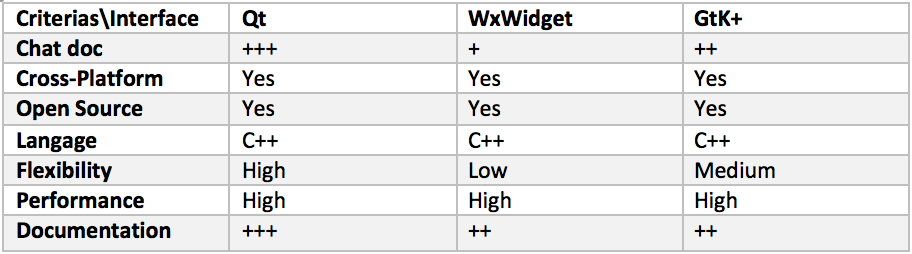
\includegraphics[width = 0.99\hsize]{./figures/comparison}
\caption{Qt, WxWidget, GTK+ comparison table}
\end{figure}
 

In order to get used to Qt, which was new to me, I have decided to complete Openclassroom tutorials [6]. Those tutorials have helped me to install QtCreator and to get familiar with Qt beginning with some basic exercices.


\clearpage
%%%%%%%%%%%%%%%%%%%%%%%%%%%%%%%%%%%%
\section{The Imaging File Format: DICOM standard }
\textbf{DICOM standard} is a special software integrated format dedicated to \textbf{ease data storage and communication} between different facilities in the \textbf{medical imaging field}. This standard has been defined by the \textbf{American College of Radiology} (ACR) and the \textbf{National Electrical Manufactural Association} (NEMA) in 1985. DICOM defines a specific data model structure, a file format and data dictionary, it also comes with a TCP/IP protocol to facilitate data transfer. Before the creation of this standard, it was challenging for distinct services to exchange imaging information, currently DICOM format is widely use among the medical imaging area. 

\newline \vspace{5mm}
DICOM standard is a well-structured but also hard to reach software. Even if its website [7] provides a wide documentation, it remains challenging to fully understand it. The aim of the following subsection is to give a basic overview of DICOM standard structures. In the scope of my project I will mainly focus on the data storage and treatment, TCP/IP protocol has not been part of my concern. Moreover, as complete the DICOM standard website could be, I used several websites [8] \& [9], to build my understanding on the DICOM file format. 





\subsection{DICOM Information Model structure}
DICOM has been created to facilitate information exchange in \textbf{the real world of patient healthcare services}, according to the medical imaging field. Hence, all information that are processed with DICOM are related to \textbf{real world elements}, that could be patient, location, studies, images etc. DICOM standard defines its own terminology to descibe the context and relationships between those element in his \textbf{DICOM Model of the Real World}, available in \textbf{\textit{Appendix 5}. From this real world model, DICOM also defines its own \textbf{Data Model Structure}. Based on the \textbf{Object Oriented Programming structure}, this data model defines \textit{Element}, generally called \textbf{DICOM Object}, that encapsulate several pieces of information. Those \textit{Element} are then grouped into \textit{Classes} depending on their similarity.

\newline \vspace{5mm}

In order to deal with data sharing, DICOM defines the \textbf{Service Class Specification}, each class being specifically related to one or more \textbf{Service Object Pair Class} (SOP). Together those classes give description of the information, roles and operations that are allowed between information-sharer. More precisely, SOP classes contain rules and semantics that organize services use. Each SOP class is made of one \textbf{Information Object Definition (IOD)} grouped with one \textbf{Service Group}. Figure 2 gives a representation of this \textbf{Information Model Structure}. 

\clearpage

\newline \vspace{5mm}

\begin{figure}[ht]
\centering
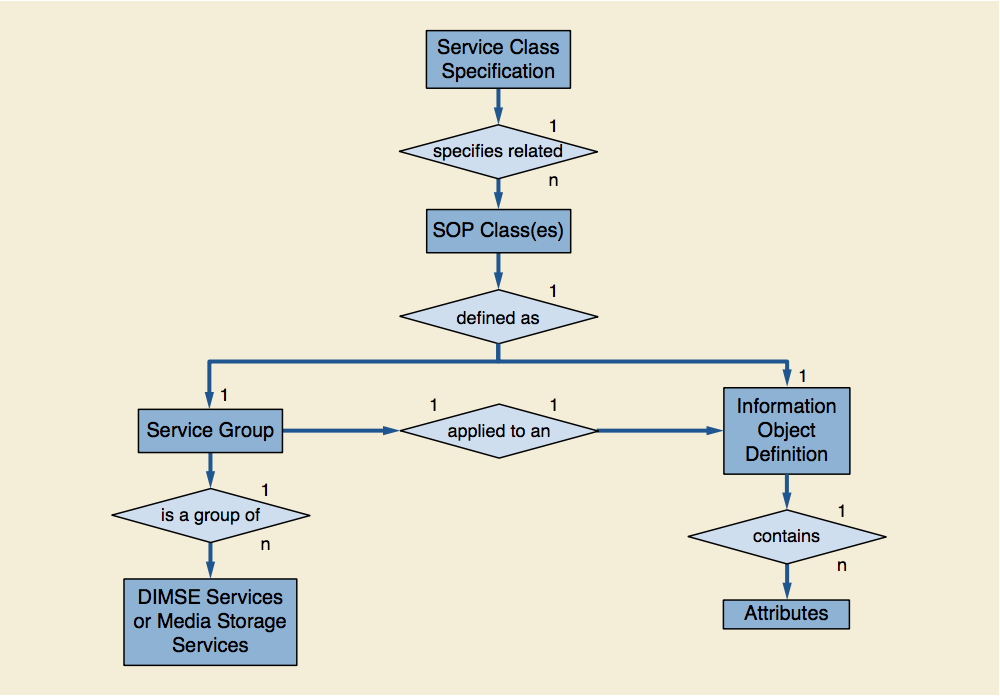
\includegraphics[width = 0.8\hsize]{./figures/DICOMInformationalModel}
\caption{DICOM Information Model Structure Representation}
\end{figure}


\begin{itemize}

\item The \textbf{DIMSE Service Group} specifies operations and notifications that are allowed on an Information Object Definition. \textbf{DIMSE} stands for DICOM Message Service Element and \textbf{Service Object Pair Classes} are used for message transfering between Information Object Definition.



\item \textbf{Information Object Definition} (IOD) are abstract objects which are intented to represent \textbf{instances of the real world model}. \textbf{Information Object Definition} can be made of one or more \textbf{Information Entities (IE)} - we talk about normalized vs composite IOD's. Each \textbf{Information Entities (IE)} and is made of \textit{attributes} describing a single piece of information. Information Entities are related to \textbf{real world object} for example a patient, and his attributes could be the patient name or date of birth. Attributes that have a link are grouped into \textbf{Information Object Module (IOM)}, which are defined in a way that they can be used in different IOD's. 

\end{itemize}


\clearpage

Figure 3 shows the representation of a Image (composite) IOD. Also, notice that all \textbf{DICOM Object} must at least contains the SOP common module and the four main \textbf{Information Entities}: Patient, Study, Serie and Image.


\newline \vspace{5mm}

\begin{figure}[ht]
\centering
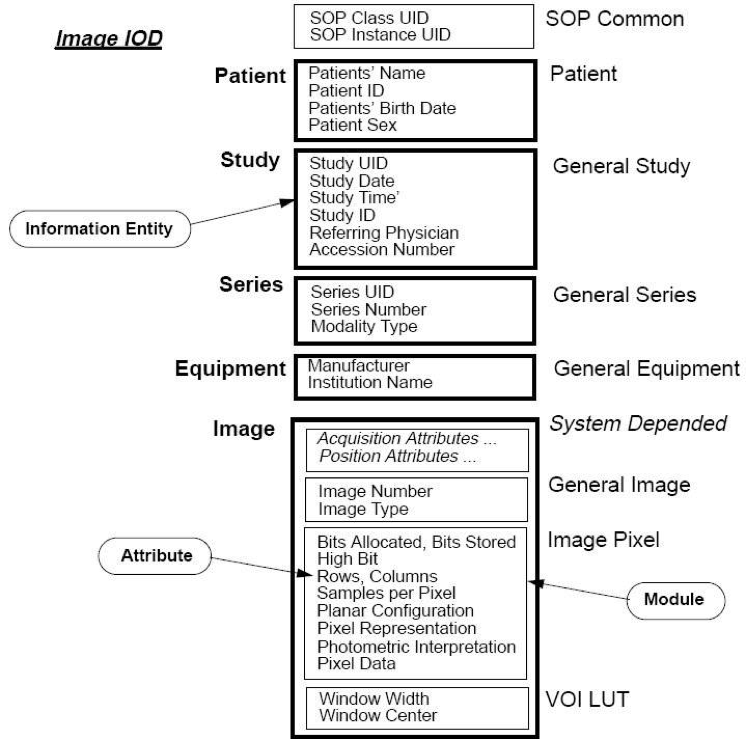
\includegraphics[width = 0.75\hsize]{./figures/ImageIOD}
\caption{Image IOD structure}
\end{figure}

\newline \vspace{5mm}

To more extend it is clear on the figure that each Information Entities has an attribute called UID, this stands for \textbf{Unique Identifier}. DICOM uses those identifiers to uniquely defines a wide variety of items to guaranty global uniqueness, mainly among different countries, sites, equipment.


\clearpage
\subsection{DICOM File Structure}
The \textbf{DICOM File Format} decribes how the information, encapsulated in an  \textbf{SOP instance}, should be stored in a byte stream, in a file on a physical medium. Each DICOM file is composed of two instance: a \textbf{Header} followed by a \textbf{Data Set}.

\begin{itemize} 
\item \textbf{The Header} contains 128 bytes preamble (which are all set to zero if it is not used) followed by 4 byte DICOM prefix (DICM). The header is not necessary included in the file but is useful to make access to data easier, indeed the prefix allows to quickly acknowledge DICOM format. Besides, no structure is required for the preamble.  

\item \textbf{The Data Set} is organised as consecutive \textbf{DICOM Data Element} (or Data Attribute), referenced in the DICOM standard [10]. Those Data Element can represent various information, from the patient name and birth to theimage pixels. More precisely one \textbf{DICOM Data Element} is \textit{one unit of information} corresponding to one encoded \textbf{Information Object Definition (IOD) Attribute}, defined above. Figure 4 gives a representation of the DICOM File structure.
\end{itemize}

\begin{figure}[ht]
\centering
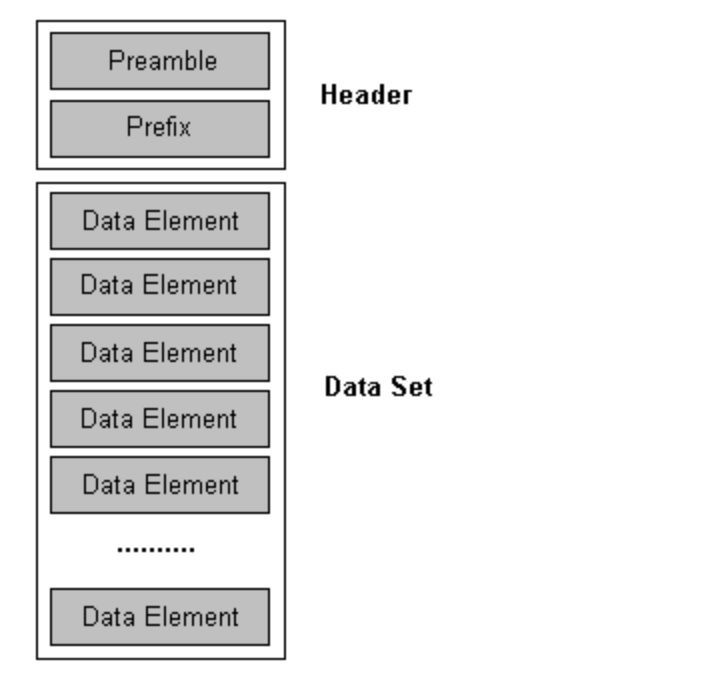
\includegraphics[width = 0.45\hsize]{./figures/DicomFileFormat}
\caption{Basic DICOM File Structure}
\end{figure}

\newline \vspace{5mm}
\textbf{DICOM Data Element} are \textit{Tag Element}, therefore DICOM can be said to be a tag file format, this mean that each element is referenced by a unique \textbf{Tag Number} defining the element and its properties. In the Data Set, Data Elements are ordered by increasing Tag Number. Each Data Element is made of the same range of consecutive fields: 
\begin{itemize} 
\item \textbf{Tag Number}: it consists in an ordered pair of 16 bits unsigned integer of the form (gggg,eeee)  representing the \textit{Group Number} - defining the Information Entity - followed by the \textit{Element Number} - defining the attribute. For example, in the tag (0028,0010), the Group Number is 0028 and correspond to the Image group, the Element Number is 0010 and correspond to the row (especially to the length of the image in pixels).
\item \textbf{Value Representation}: it defines the data type of the element. As the Tag Number already implies the data type, the value representation can be omitted.
\item \textbf{Value Length}: either 16 or 32 bits element, this defines the length of the following value.
\item \textbf{Value Field}: consists in an even number of bytes containing the value of the element; this field can contain the Value Multiplicity, which would specified the number of values that can be encoded in the field. 
\end{itemize}

\begin{figure}[ht]
\centering
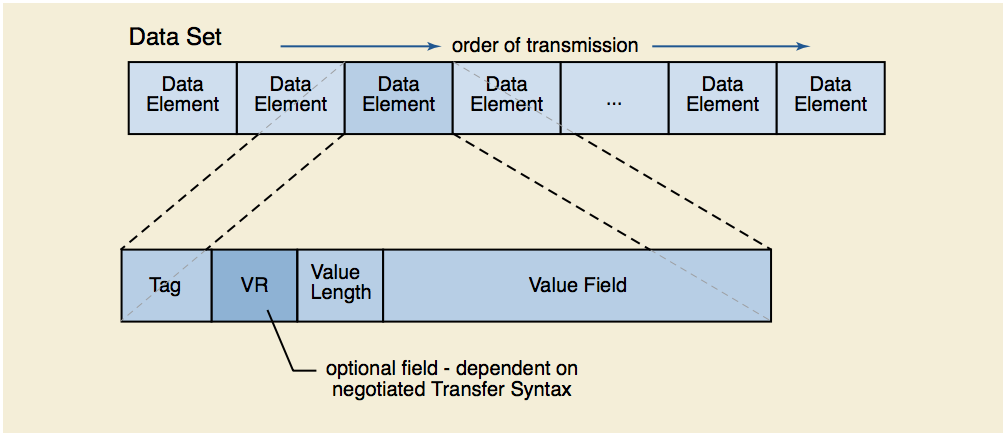
\includegraphics[width = 0.8\hsize]{./figures/DataSetandDataElement}
\caption{Data Set and Data Element structure}
\end{figure} 



\clearpage
\subsection{DICOM Folder - Patient level}
While asking for their medical imaging data, patients will be given a \textbf{DICOM Folder} containing all relevant information. Every basic DICOM folder should contain one DICOM element called \textbf{DICOMDIR} and a folder named \textbf{DICOMDAT} leading path to the images.

 
\begin{itemize}
\item From the DICOMDAT folder, the hierachical structure will be as follow:

\begin{forest}
  for tree={
    font=\ttfamily,
    grow'=0,
    child anchor=west,
    parent anchor=south,
    anchor=west,
    calign=first,
    edge path={
      \noexpand\path [draw, \forestoption{edge}]
      (!u.south west) +(7.5pt,0) |- node[fill,inner sep=1.25pt] {} (.child anchor)\forestoption{edge label};
    },
    before typesetting nodes={
      if n=1
        {insert before={[,phantom]}}
        {}
    },
    fit=band,
    before computing xy={l=15pt},
  }
[DICOMDAT
  [\textbf{SDY00000}
    [\textit{SRS00000}
		[IMG00000]
		[...]
		[IMG0000N]
	
	]
    [\textit{SRS00001}
		[IMG00000]
		[...]
		[IMG0000N]
	]
	
    [\textit{SRS00002}]
  ]
  [\textbf{SDY00001}
    [\textit{SRS00000}]
  ]
]
\end{forest}

\begin{itemize}
	\item \textbf{SDY0000} folder represents a unique study for a given patient. One study correspond to one set of exams, on request of the patient to explore on part of the body at a given time. A study can be made of one or more series.
	\item \textbf{SRS0000} stands for a unique serie. One serie correspond to a specific exam organisation (patient orientation, duration, etc.) used to capture the image(s). A serie can be made of one or more images.
	\item \textbf{IMG00000} are DICOM Images Element, corresponding to the propper "Medical Images". Those elements contain all the relevant information that should be used to render the images on a screen.
	
\end{itemize}
	

\item The \textbf{DICOMDIR} is a \textbf{DICOM File Object} containing the tree structure described above. This will allow to automatically get the path to each element. It also contains the general information according the the exam (patient information, study ID, date). 
\end{itemize}

The folder might contain other non DICOM element (e.g the report) that won't be recorded by the DICOMDIR. During the creation of my interface, this DICOMDIR has allow me to browse through all the folder element and to automatically find path to images.





\clearpage

%%%%%%%%%%%%%%%%%%%%%%%%%%%%%%%%%%%%
\section{Classes and File Structure}
\textbf{DICOM standard} is a special software integrated format dedicated to \textbf{ease data storage and communication} between different facilities in the \textbf{medical imaging field}. This standard has been defined by the \textbf{American College of Radiology} (ACR) and the \textbf{National Electrical Manufactural Association} (NEMA) in 1985. DICOM defines a specific data model structure, a file format and data dictionary, it also comes with a TCP/IP protocol to facilitate data transfer. Before the creation of this standard, it was challenging for distinct services to exchange imaging information, currently DICOM format is widely use among the medical imaging area. 

\newline \vspace{5mm}
DICOM standard is a well-structured but also hard to reach software. Even if its website [7] provides a wide documentation, it remains challenging to fully understand it. The aim of the following subsection is to give a basic overview of DICOM standard structures. In the scope of my project I will mainly focus on the data storage and treatment, TCP/IP protocol has not been part of my concern. Moreover, as complete the DICOM standard website could be, I used several websites [8] \& [9], to build my understanding on the DICOM file format. 




\subsection{DCMTK Library and Qt}
\textbd{DCMTK} is an \textbf{open-source} collection of libraries and scripts that has been made to deals with  \textbf{DICOM Objects}. This toolkit is widely used by hospitals, companies or private individuals, that aim at creating DICOM-related desktop software. DCMTK provides already built \textbf{DICOM-related classes} suitabely made to treat, construct, and convert DICOM objects; it also provides an internal worklist server in order store, send or receive images. DCMTK source code repository is available on Github and free for downloading and is available for both Windows and Unix operating systems. 


\newline \vspace{5mm}


What I want to tell:

1. Why I choose dcmtk: 
 obviously I coudln't unwrap dicom element by myself
 dcmtk provided me a way to access tag element easily
 sound's widely used on the internet --> lot's of prebuild readers were using dcmtk


\newline \vspace{5mm} 
 
2. Building dcmtk:
 issues 
 solutions --> explain how to link 
 
 
3. Dcmtk classes 

As I said DCMTK provides well-formed classes

had to go through dcmtk documentation to find the relevant function I will use ! 

Dcmtk provides a lot a classes to deal with dicom format 


Developp the one I used:

- DicomImages
- Dealing with tag element -> file and get bordel
- DICOM bordel going though the tree 
	

\clearpage
\subsection{Classes and UML Diagram}
Explain the code file structure 

UML diagramm of the class (without all attribute for serie and maine window)

Explain the approach

Class definition

 screenshot for serie and Mainwindow.h in appendix Serie Class Definition and MainWindow Class definition


\clearpage
%%%%%%%%%%%%%%%%%%%%%%%%%%%%%%%%%%%%
\section{Implementation}
\textbf{DICOM standard} is a special software integrated format dedicated to \textbf{ease data storage and communication} between different facilities in the \textbf{medical imaging field}. This standard has been defined by the \textbf{American College of Radiology} (ACR) and the \textbf{National Electrical Manufactural Association} (NEMA) in 1985. DICOM defines a specific data model structure, a file format and data dictionary, it also comes with a TCP/IP protocol to facilitate data transfer. Before the creation of this standard, it was challenging for distinct services to exchange imaging information, currently DICOM format is widely use among the medical imaging area. 

\newline \vspace{5mm}
DICOM standard is a well-structured but also hard to reach software. Even if its website [7] provides a wide documentation, it remains challenging to fully understand it. The aim of the following subsection is to give a basic overview of DICOM standard structures. In the scope of my project I will mainly focus on the data storage and treatment, TCP/IP protocol has not been part of my concern. Moreover, as complete the DICOM standard website could be, I used several websites [8] \& [9], to build my understanding on the DICOM file format. 




\subsection{Rendering DICOM Images}
The first challenge of this project was to render a set of DICOM Images or at least one DICOM Image. 

As I already explained, in part 4.4, the DICOM folder tree structure blablabla 


However IMG0000 file are not of only one type, this file can be either:
\begin{itemize}
	\item One single frame DICOM Image
	\item Several single frame DICOM Images
	\item One multiframe DICOM Image
\end{itemize}

Objectively, single and multi frame images only differ by the size of the file.

\newline \vspace{5mm}	
\textbf{1. Display one image:}

\newline \vspace{5mm}	

The DCMTK library that I installed contains several classes that should make DICOM Images treatment easier.
The class I used to deal with DICOM Images files is called DicomImage, the class structure and related functions are available on DCMTK website [8888].
The class is provided with four different constructors and depending on the given parameters this class allows to deal with single frame and multiframe images. Information about the constructor I choosed are available on Appendix XXX figure YYY


\begin{itemize}
	\item Display single frame DICOM Image:
	
	\begin{center}
	\textit{DicomImage *DcmImg = new DicomImage(path)}
	\end{center}
	
	
	\item Display multiframe DICOM Image:
	
	\begin{center}
	\textit{DicomImage *DcmImg = new DicomImage(path,0,index,1)}
	\end{center}
	
	\textit{index} being the index of the frame to display
	
\end{itemize}

The variable \textit{path} is a string and contains the absolut path to the DICOM Image file.
\newline \vspace{5mm}


Once I got the DicomImage object, I need to get the pixels in order to have the opportunity to use QImage class thereafter. Here again DCMTK provide me with the function \textit{getOutputData()} - see Appendix XX figure ZZ -. The corresponding line of code is:
\newline \vspace{5mm} 

	\begin{center}
	\textit{uint8_t* pixelData= DcmImg->getOutputData(8)}
	\end{center}

\newline \vspace{5mm}  
Explain what is uint8_t



Finally I only need to use two classes provided by Qt to render the DICOM Image on my application:

\newline \vspace{5mm} 

	\begin{center}
	\textit{uint8_t* pixelData= DcmImg->getOutputData(8)}
	\end{center}

\newline \vspace{5mm}  

QIMage only takes pixel and a scene can only display QPixmap element see appendix


\newline \vspace{5mm}	

\textbf{2. Store and display successive images of the serie}

\newline \vspace{5mm}	






\clearpage
\subsection{Building 3D plan}
\input{src/section/implementation/orthogonalplan}



\clearpage
%%%%%%%%%%%%%%%%%%%%%%%%%%%%%%%%%%%%


\section{Results}
As specified at the begining of this report, the main goal of my project was to build a Graphical User Interface, suitably made for medical imaging patient in order to help them view their medical images. The final result of my project consist consequently in a Windows runnable application, that can be used by anyone, in order to view imaging data. The following section will present the finale output of the interface in terms of content and features. The first part intend to give a general overview of the interface, describing the different steps from the launching of the app to the effective display of one medical image. The second part will focus more precicesly on the features that I have developped and are available through the interface.
\subsection{Interface Overview - General Content}
From the launch of the app through the effective display of the \textit{MainWindow}, the user will first have to come accross several steps/windows that are described below:

\begin{itemize}
	\item \textbf{Welcome page and Disclaimer}:
	
	\newline \vspace{3mm} 
	
	The first contact with the interface consist in a \textit{Welcoming Page} explaining the utility of the interface. User will get indication about the way of accessing his images and will be given a disclaimer, as follow:
	
	\newline \vspace{3mm}  
	
	``
	\textbf{Welcome} \\ 
	This interface is designed for patients to view their medical images. \\
	Please select the file corresponding to the study you wish to view (select folder SDY00XXX). \\
	Your images are protected by PIN.  \\
	Your pin is your date of birth in the following format: YYYY/MM/JJ
	
	\newline \vspace{3mm}  
	
	
	\textbf{Disclaimer:}
	\begin{itemize}
		\item These images are for information only 
		\item Do not try to interpret your images 
		\item For any queries, please contact your healthcare professional 
		\item Some people may find seeing images of themselves upsetting, please consider whether you want to view them 
		\item Be aware that these images constitute your personal medical data - please be mindful of who you share them with
	\end{itemize}''
	
	
	
	\newline \vspace{3mm}  
	
	An overview of this \textbf{Welcome Page} is available in \textbf{\textit{Appendix 9}}. This page is supported by a button \textit{Select File} to allow the user to choose the study he wish to display on the screen. By default the first image displayed will be the first image of the first serie.
	 
	 \clearpage
	
	\item \textbf{PIN Access}: 
	
	\newline \vspace{3mm} 
	
	As the interface is dealing with sentitive medical data, images won't show automatically once selected. Indeed, data are protected by a PIN access, which correspond, as described in the disclaimer, to the patient date of birth in the format YYYY/MM/JJ; an overview of this window is available on \textbf{\textit{Appendix 10 figure 18}}. If the PIN provided is not right, the user will be informed on his screen and have the right to write another code, see \textbf{\textit{Appendix 10, figure 19}}. If no PIN in provided and the window is closed by the user, the application will close automatically. However, if the user provide the right PIN, he will have access to his images and the Main Window will pop up.
	
	
	\item \textbf{Main Window}:
	
	\newline \vspace{3mm} 
	
	The \textit{MainWindow} is the heart of the interface, this is the window that will allow the user to view his images and select options. An overview of the screen is available on \textbf{\textit{Appendix 11}}, displaying the CT-scan of an abdomen. The architecture of this interface has been realized taking inspiration on the \textbr{Interface Design Specification} (Appendix 4) mentionned in part 3.1. All the available features concerning images treatment and information access will be described in the following part.
		
	
\end{itemize}

\clearpage
\subsection{Available features}
\newcommand{\IconZoom}{
\includegraphics[width=1em]{figures/icon/zoom-plus}}
\newcommand{\IconFlag}{
\includegraphics[width=1em]{figures/icon/flag}}
\newcommand{\IconOneWindow}{
\includegraphics[width=1em]{figures/icon/w4}}
\newcommand{\IconFourWindow}{
\includegraphics[width=1em]{figures/icon/w1}}
\newcommand{\IconPlan}{
\includegraphics[width=1em]{figures/icon/sagittal}}
\newcommand{\IconScroll}{
\includegraphics[width=1em]{figures/icon/scroll}}
\newcommand{\IconLink}{
\includegraphics[width=1em]{figures/icon/link}}
\newcommand{\IconContrast}{
\includegraphics[width=1em]{figures/icon/defaultcontrast}}
\newcommand{\IconNormal}{
\includegraphics[width=1em]{figures/icon/examples}}

\begin{itemize}
	\item {\IconZoom} \textbf{Zoom in/out}:
	
	\newline \vspace{3mm} 
	
	User can choose to Zoom in/out on the current selected image in order to reach more details, or simply to adapt the image to the window.
	
	\item {\IconFlag} \textbf{Display Flagged Image(s)}: 
	
	\newline \vspace{3mm} 
	
	The Flagged Image(s) of a serie correspond to the most ``relevant'' one and is supposed to give more precision about the condition of the patient - see appendix XXX. This kind of Image has to be directly inserted in the DICOM file, at the right place corresponding the the serie within a study. Path will be of the form ``FLAGGED/SDY00000/SRS00000/FLAG1.png''. There can be one or more Flagged Images and the path will be directly found by the app.
	\item {\IconFourWindow} \textbf{Display one or more window}:
	
	\newline \vspace{3mm} 
	
	Interface-user can choose to display one, two or four window on the screen depending on the number of serie he wants to watch.
	
	\item {\IconOneWindow} \textbf{Choose the serie(s) to display}:
	
	\newline \vspace{3mm}
	
	One can choose which serie to display in which window. For the moment he can only display several series from the same study. See appendix XX.
	
	\item {\IconPlan} \textbf{Choose the plan to display}:
	
	\newline \vspace{3mm}
	
	As described in the section 5.2, for series where the set of images is large enough, and the algorithm has been able to define the default plan of the images, the algorithm is able to recreate the two other corresponding plan of the serie. When enabled, the patient can choose which plan to display in the current window.
	
	\item {\IconScroll} \textbf{Scroll Images}:
	
	\newline \vspace{3mm}
	
	For series containing more thant one image, by default while using the mouse wheel, the interface will display successively the images of the serie.
	
	\item {\IconLink} \textbf{Link Scrolling}:
	
	\newline \vspace{3mm}
	
	If the algorithm has been able to construct all the 3 plan from the given serie (section 5.2) and the user has choosen to display at least two plan on the same serie, it is possible for him to link the scroll of images. Linking scroll meaning display a red line that will inform about the position on the current image in the other plan, result is available on appendix XX. By default, window displaying the same plan of the same serie will scroll all at once.
	
	\item {\IconContrast} \textbf{Display different contrast}:
	
	\newline \vspace{3mm}
	
	DICOM provides 3 already made level of contrast call in their term ``Windowing'', ``MinMax'', and ``Histogram''. I replace the terms in Default, Darker and Brighter contrast. By clicking on the corresponding button, one can choose to display the serie in a different contrast, the appendix XX show an exemple of the several contrast that can be displayed. I also add the possibility for each of this contrast, to invert the grayscale of the image. At the moment, for multiplan series, changing the contrast on one of the plan will change it for all of the corresponding plan (storrage concern). 
	
	\item {\IconContrast} \textbf{Compare to ``Normal'' Images}:
	
	\newline \vspace{3mm}
	
	If the result of the exam show that the patient is not in a ``normal'' condition, example of normal images will be provided in the given file. On the same principe as Flagged Images, these images need to be inserted by a clinician, using a path of the form ``REFERENCES/SDY00000/SRS00000/REF1.png''
	
	\item \textbf{Access to reports}
	
	\newline \vspace{3mm}
	
	Clicking on the relative button, user will be given access to his both \textit{clinical} and \textit{simplified} report. Those report have to be filled by a clinician and given to a jpeg format (for the moment), using a path of the form ``REPORTS/SDY00000/CLINICALREPORT.jpeg''. The reports will appear in a distinct designated window, the patient can decide wether he want's to display only on of those reports or both at the same time. An overview of this window in available on \textbf{\textit{Appendix 12}}.

 
\end{itemize}






\clearpage
%%%%%%%%%%%%%%%%%%%%%%%%%%%%%%%%%%%%


\section{Evaluation}
\textbf{DICOM standard} is a special software integrated format dedicated to \textbf{ease data storage and communication} between different facilities in the \textbf{medical imaging field}. This standard has been defined by the \textbf{American College of Radiology} (ACR) and the \textbf{National Electrical Manufactural Association} (NEMA) in 1985. DICOM defines a specific data model structure, a file format and data dictionary, it also comes with a TCP/IP protocol to facilitate data transfer. Before the creation of this standard, it was challenging for distinct services to exchange imaging information, currently DICOM format is widely use among the medical imaging area. 

\newline \vspace{5mm}
DICOM standard is a well-structured but also hard to reach software. Even if its website [7] provides a wide documentation, it remains challenging to fully understand it. The aim of the following subsection is to give a basic overview of DICOM standard structures. In the scope of my project I will mainly focus on the data storage and treatment, TCP/IP protocol has not been part of my concern. Moreover, as complete the DICOM standard website could be, I used several websites [8] \& [9], to build my understanding on the DICOM file format. 




\subsection{Lay person evaluation}
\input{src/section/evaluation/patienteval}


\clearpage
\subsection{Ethic and LSEPI checklist}
\input{src/section/evaluation/lsepi}

\clearpage
\subsection{Personal evaluation}
--> explain some choice 
\newline
--> show calcul for different plan output


\clearpage
%%%%%%%%%%%%%%%%%%%%%%%%%%%%%%%%%%%%
\section{Conclusions and Future work}
\input{src/section/conclusionandfuture/conclusion}


Remaining tasks 

\begin{itemize}
	\item reset button
	\item anonymize and share 
	\item possibility to open another study 
	\item take comments into consideration

\end{itemize}


\clearpage
%%%%%%%%%%%%%%%%%%%%%%%%%%%%%%%%%%%%
\section{Appendix}
\clearpage

\subsection {Appendix 1 - Expert Questionnaire Results from William PhD}
\begin{figure}[ht]
\centering
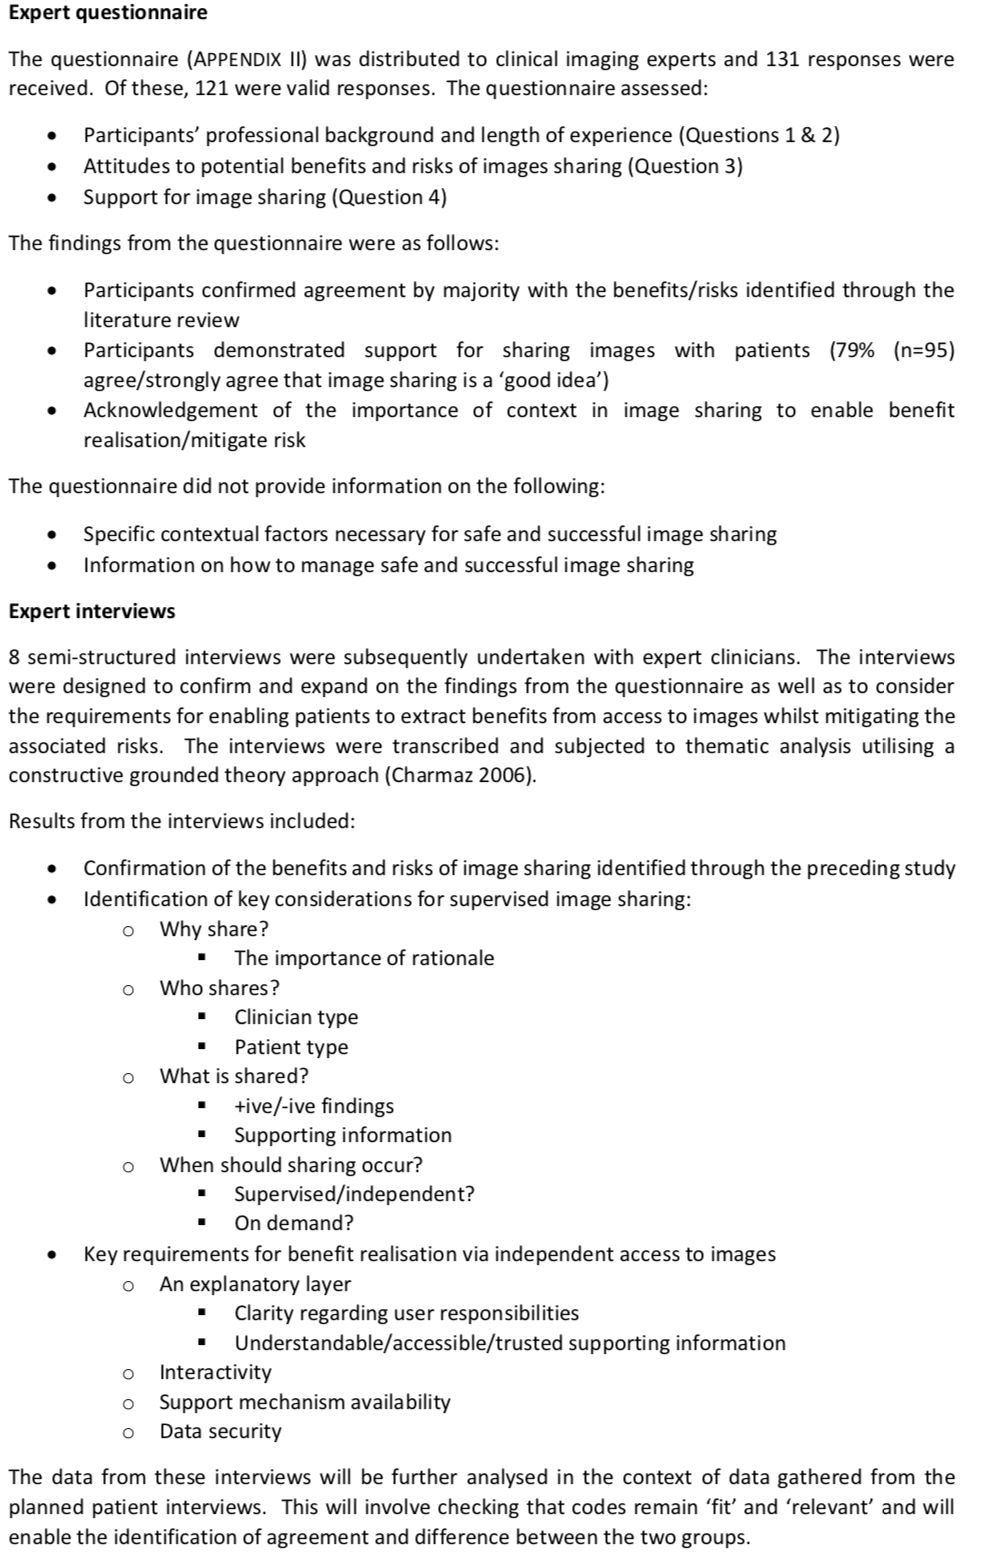
\includegraphics[width = 0.80\hsize]{./figures/ExpertResult}
\caption{Expert Questionnaire Results}
\end{figure}

\clearpage

\subsection {Appendix 2 - General Specification}
\begin{figure}[ht]
\centering
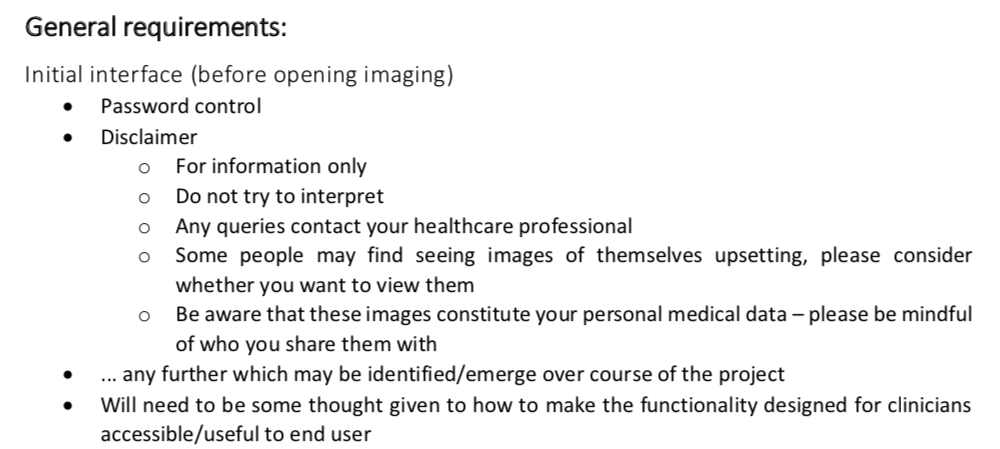
\includegraphics[width = 0.95\hsize]{./figures/GeneralSpec1}
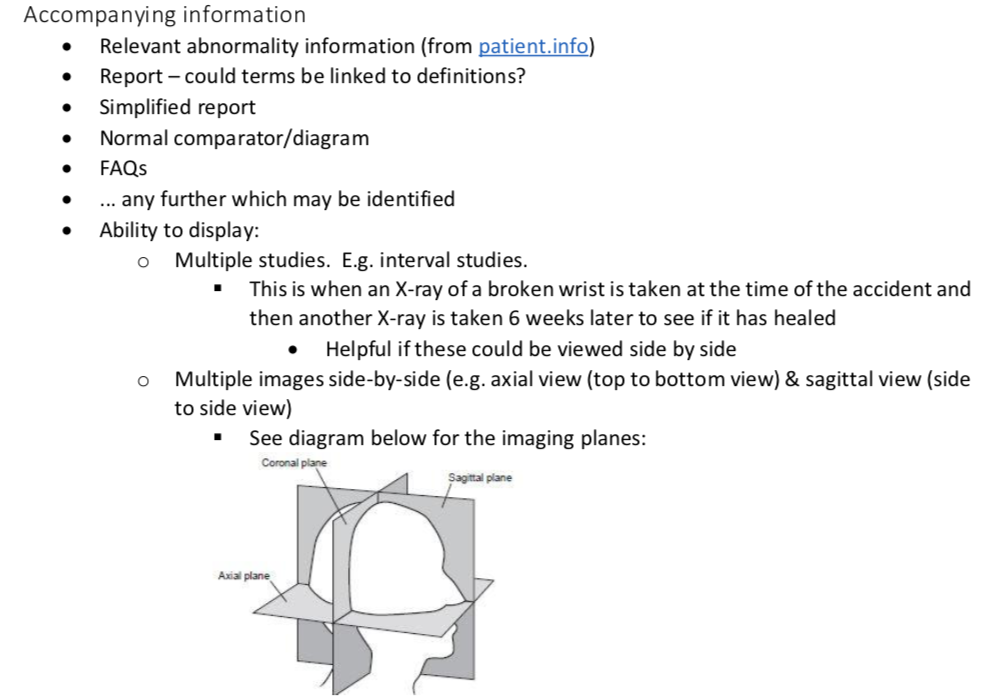
\includegraphics[width = 0.95\hsize]{./figures/GeneralSpec2}
\end{figure}



\clearpage

\begin{figure}[ht]
\centering
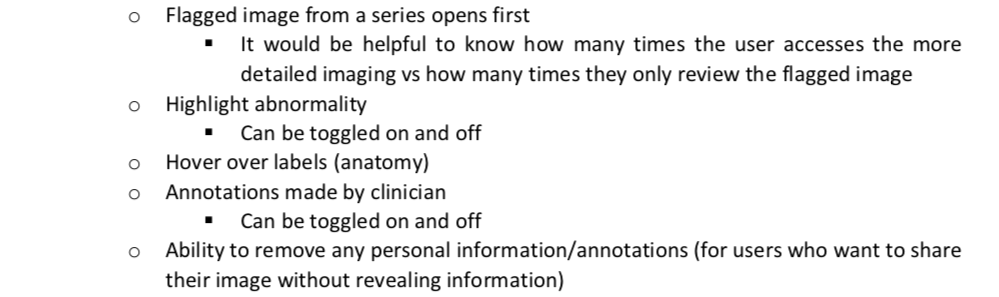
\includegraphics[width = 0.95\hsize]{./figures/GeneralSpec3}
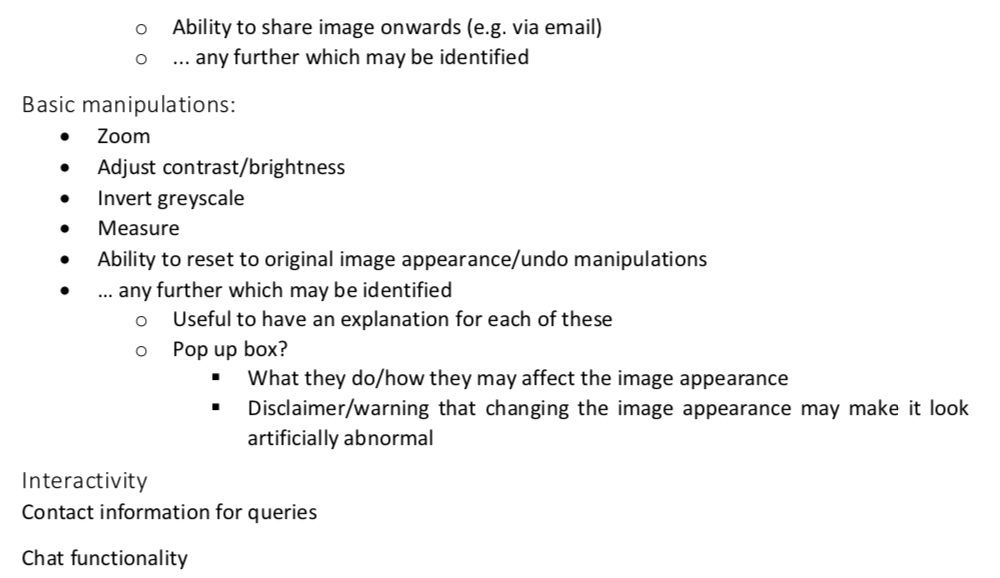
\includegraphics[width = 0.95\hsize]{./figures/GeneralSpec4}
\end{figure}

\clearpage

\subsection {Appendix 3 - Imaging Specification}
\begin{figure}[ht]
\centering
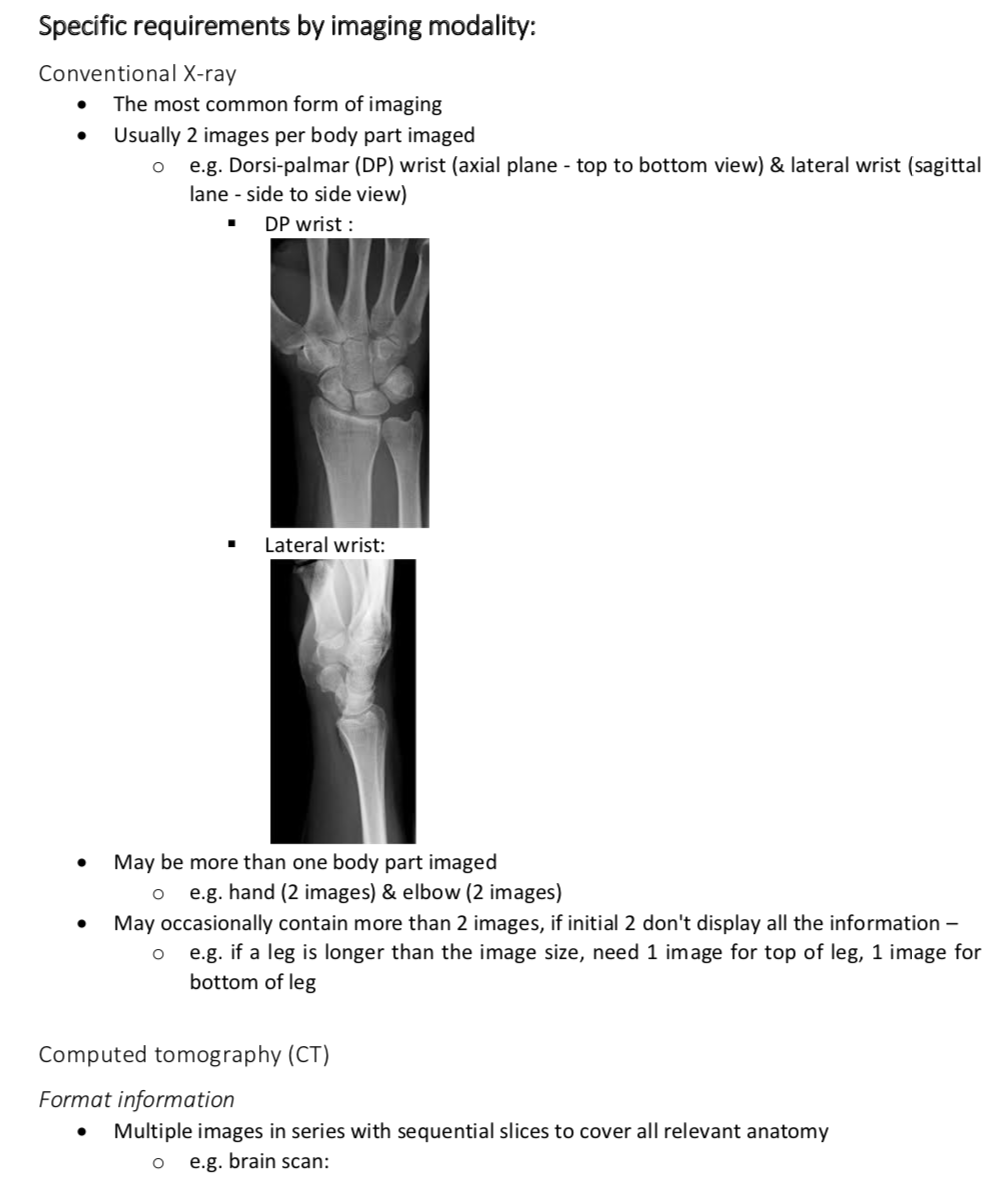
\includegraphics[width = 0.93\hsize]{./figures/ImagingSpec1}
\caption{Imaging Specification 1}
\end{figure}
\clearpage

\begin{figure}[ht]
\centering
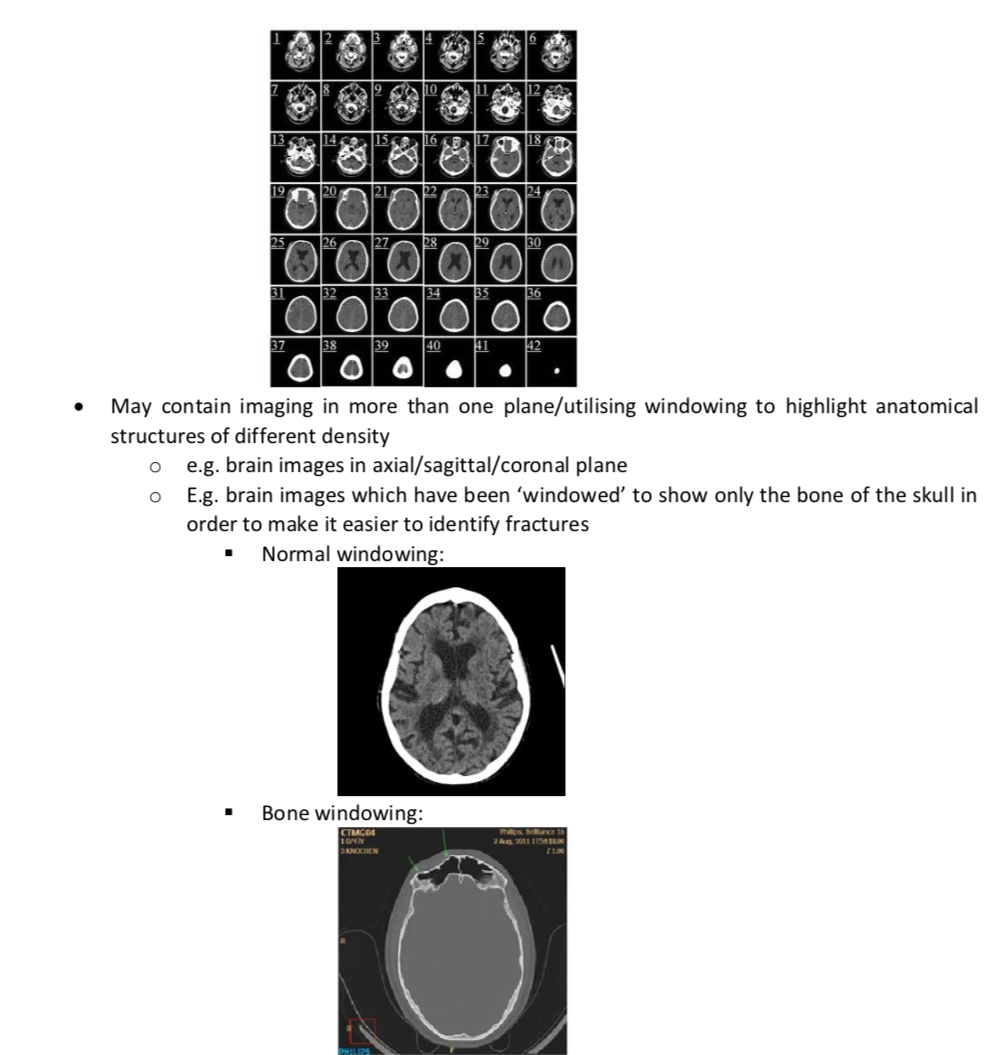
\includegraphics[width = 0.95\hsize]{./figures/ImagingSpec2}
\caption{Imaging Specification 2}
\end{figure}
\clearpage

\begin{figure}[ht]
\centering
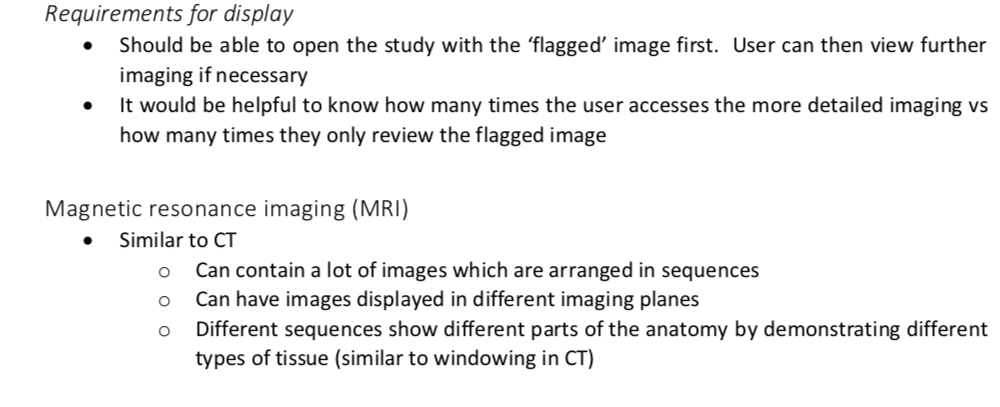
\includegraphics[width = 0.95\hsize]{./figures/ImagingSpec3}
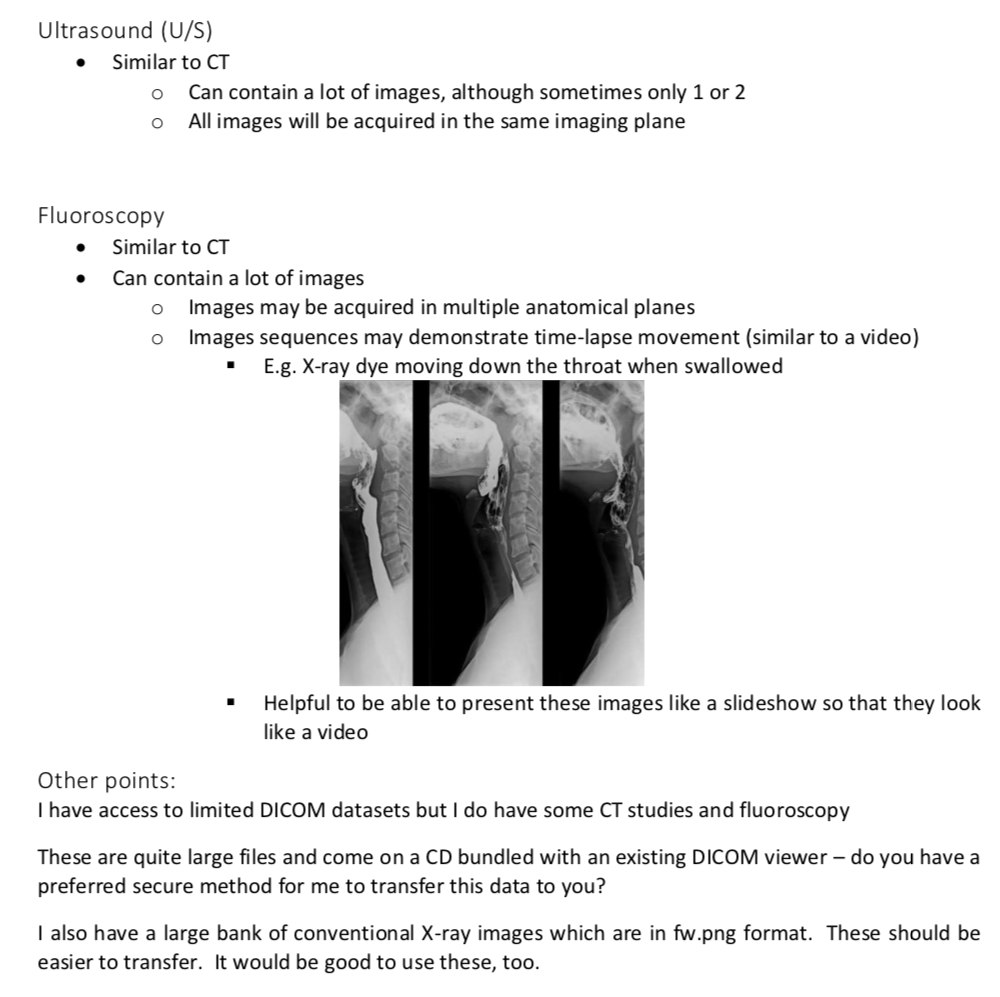
\includegraphics[width = 0.95\hsize]{./figures/ImagingSpec4}
\caption{Imaging Specification 3}
\end{figure}



\clearpage
\subsection {Appendix 4 - Interface Design Specification}
\begin{figure}[ht]
\centering
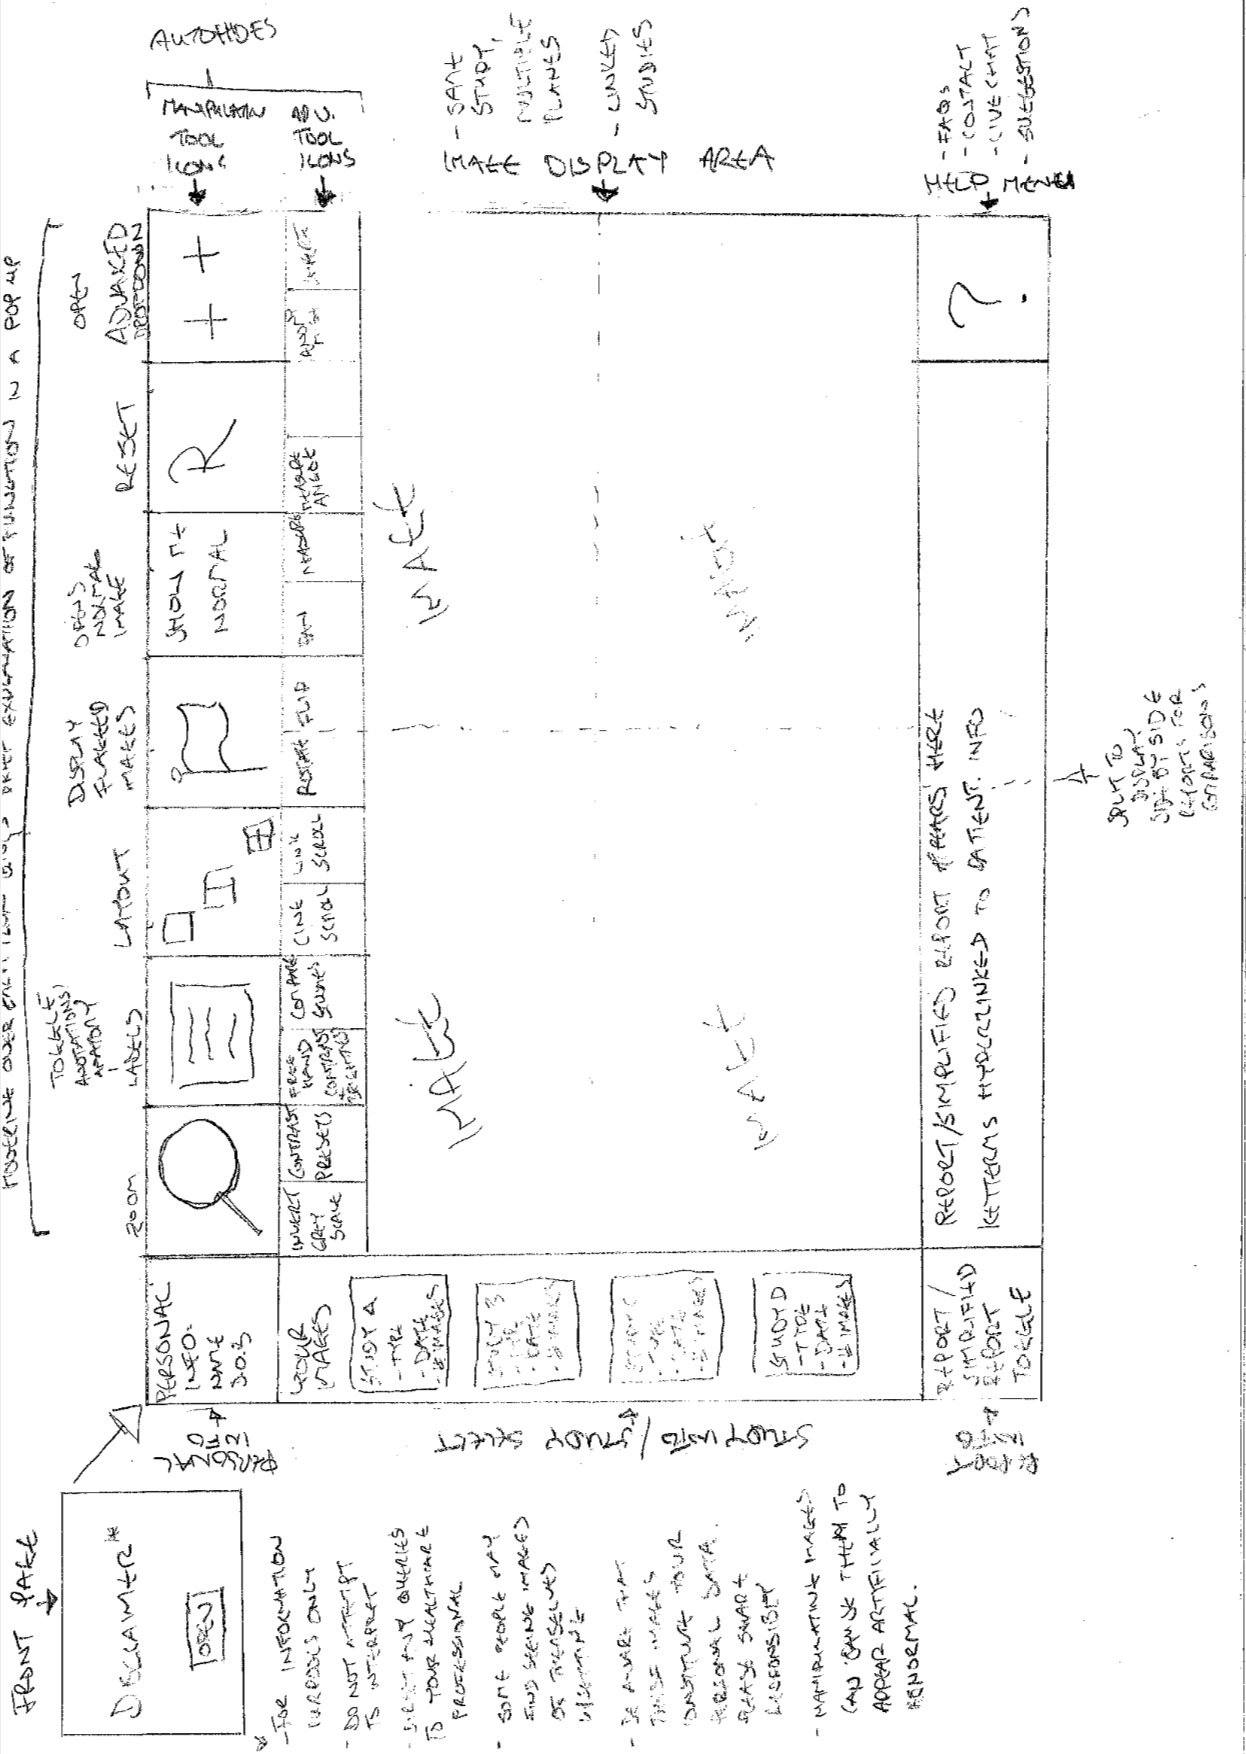
\includegraphics[width = 0.80\hsize]{./figures/InterfaceDesign}
\caption{Interface Design - Drawing Specification}
\end{figure}

\begin{figure}[ht]
\centering
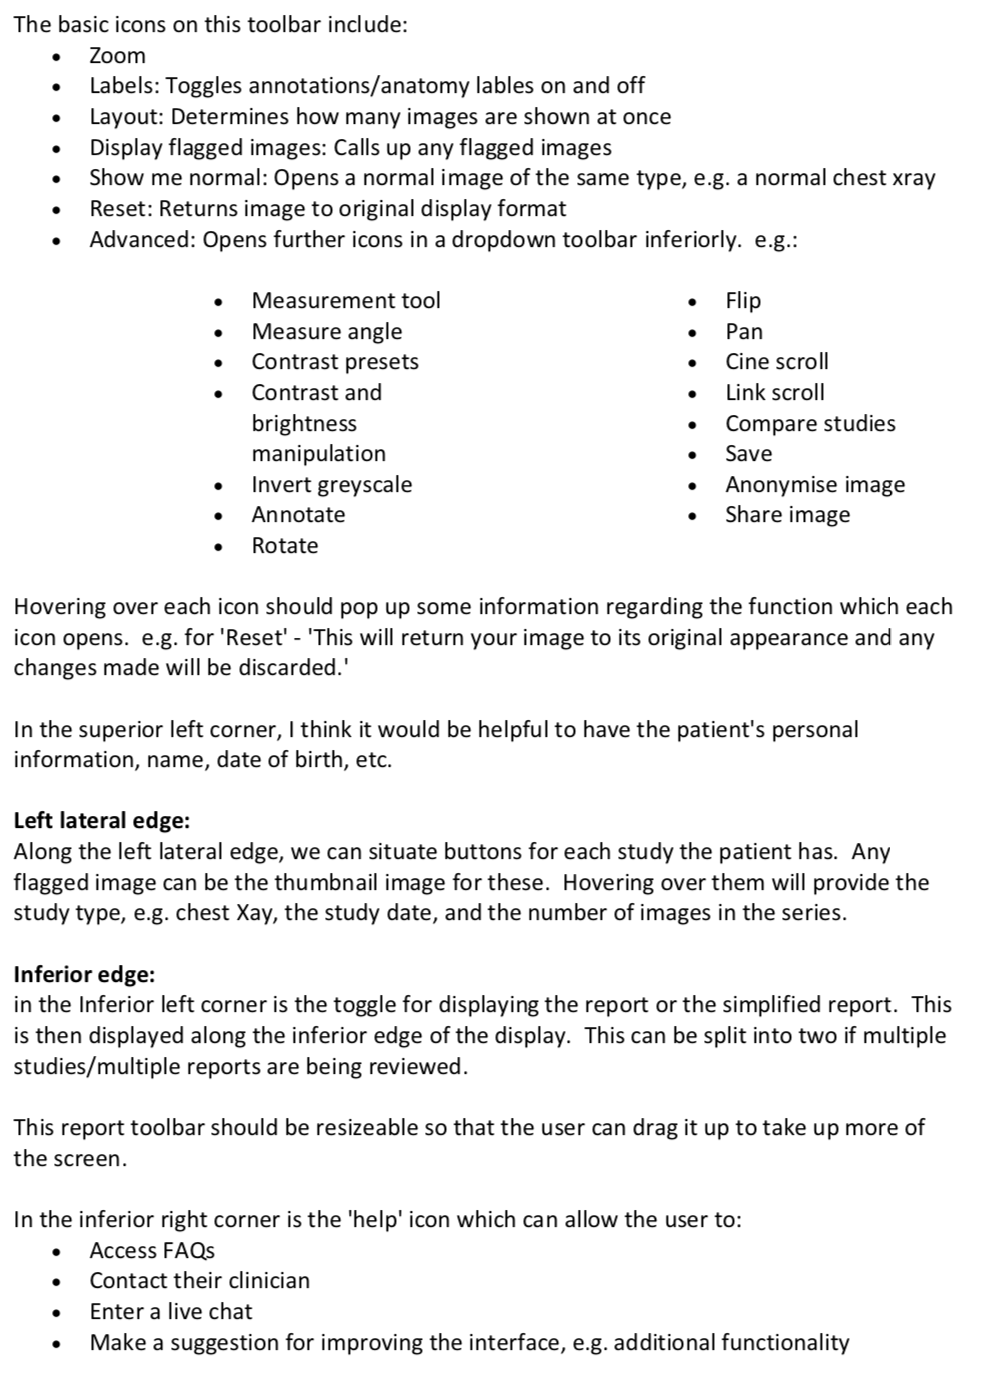
\includegraphics[width = 0.80\hsize]{./figures/DesignSpec}
\caption{Interface Design - Features Specification}
\end{figure}

\clearpage

\subsection {Appendix 5 - DICOM model of the Real World}
\begin{figure}[ht]
\centering
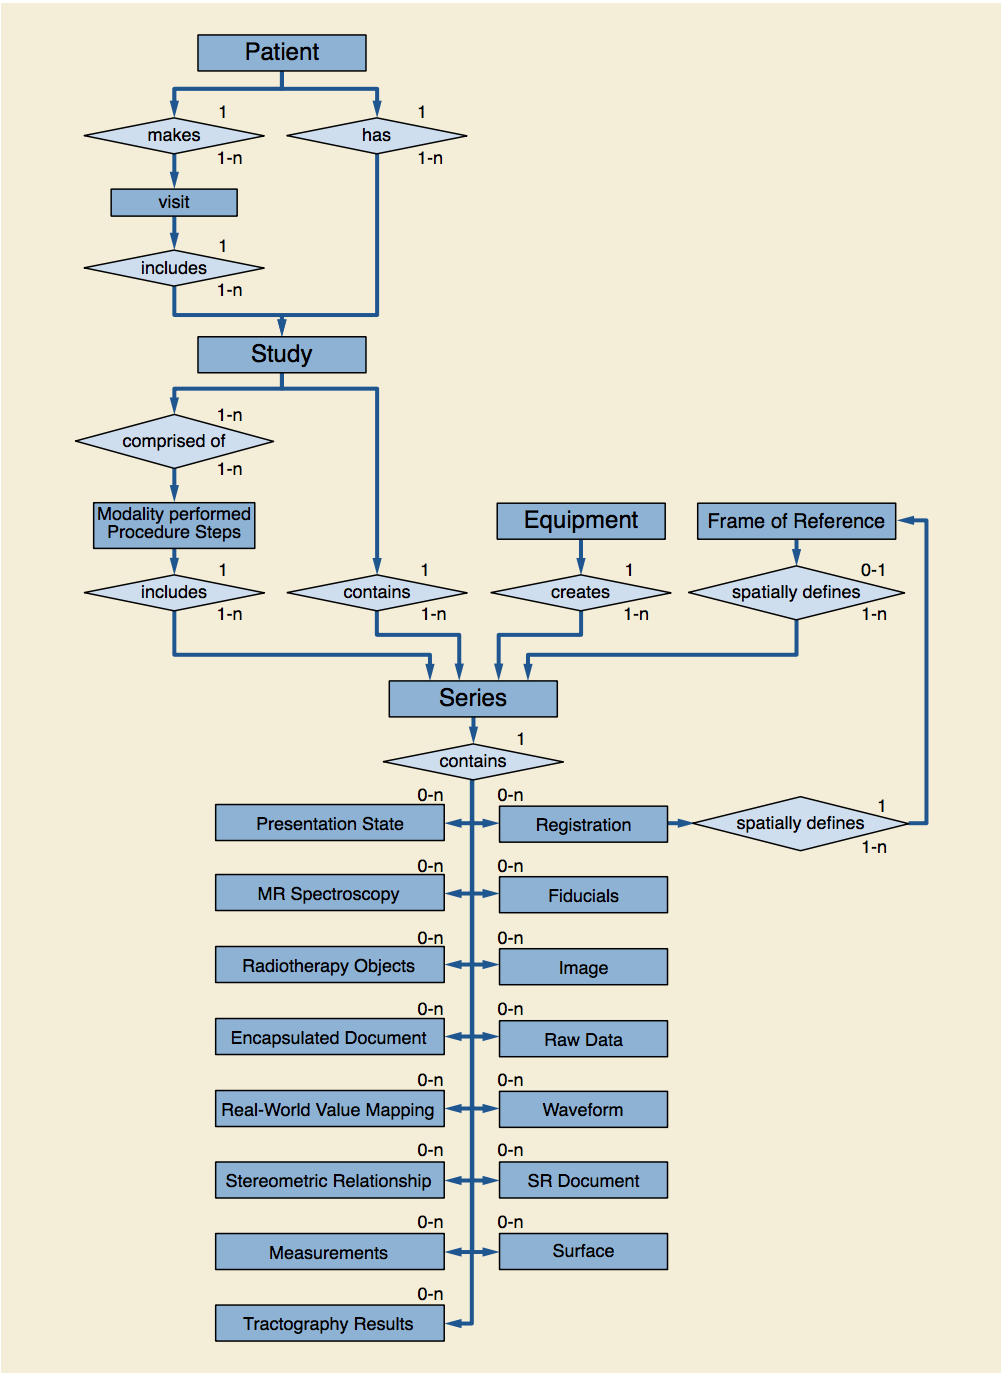
\includegraphics[width = 0.83\hsize]{./figures/DICOMRealWorldModel}
\caption{DICOM Model of the Real World}
\end{figure}

\clearpage

\subsection {Appendix 6 - UML Diagram}
%\input{src/appendix/}

\clearpage

\subsection {Appendix 7 - DCMTK: Relevant classes and functions declarations}
\begin{figure}[ht]
\centering
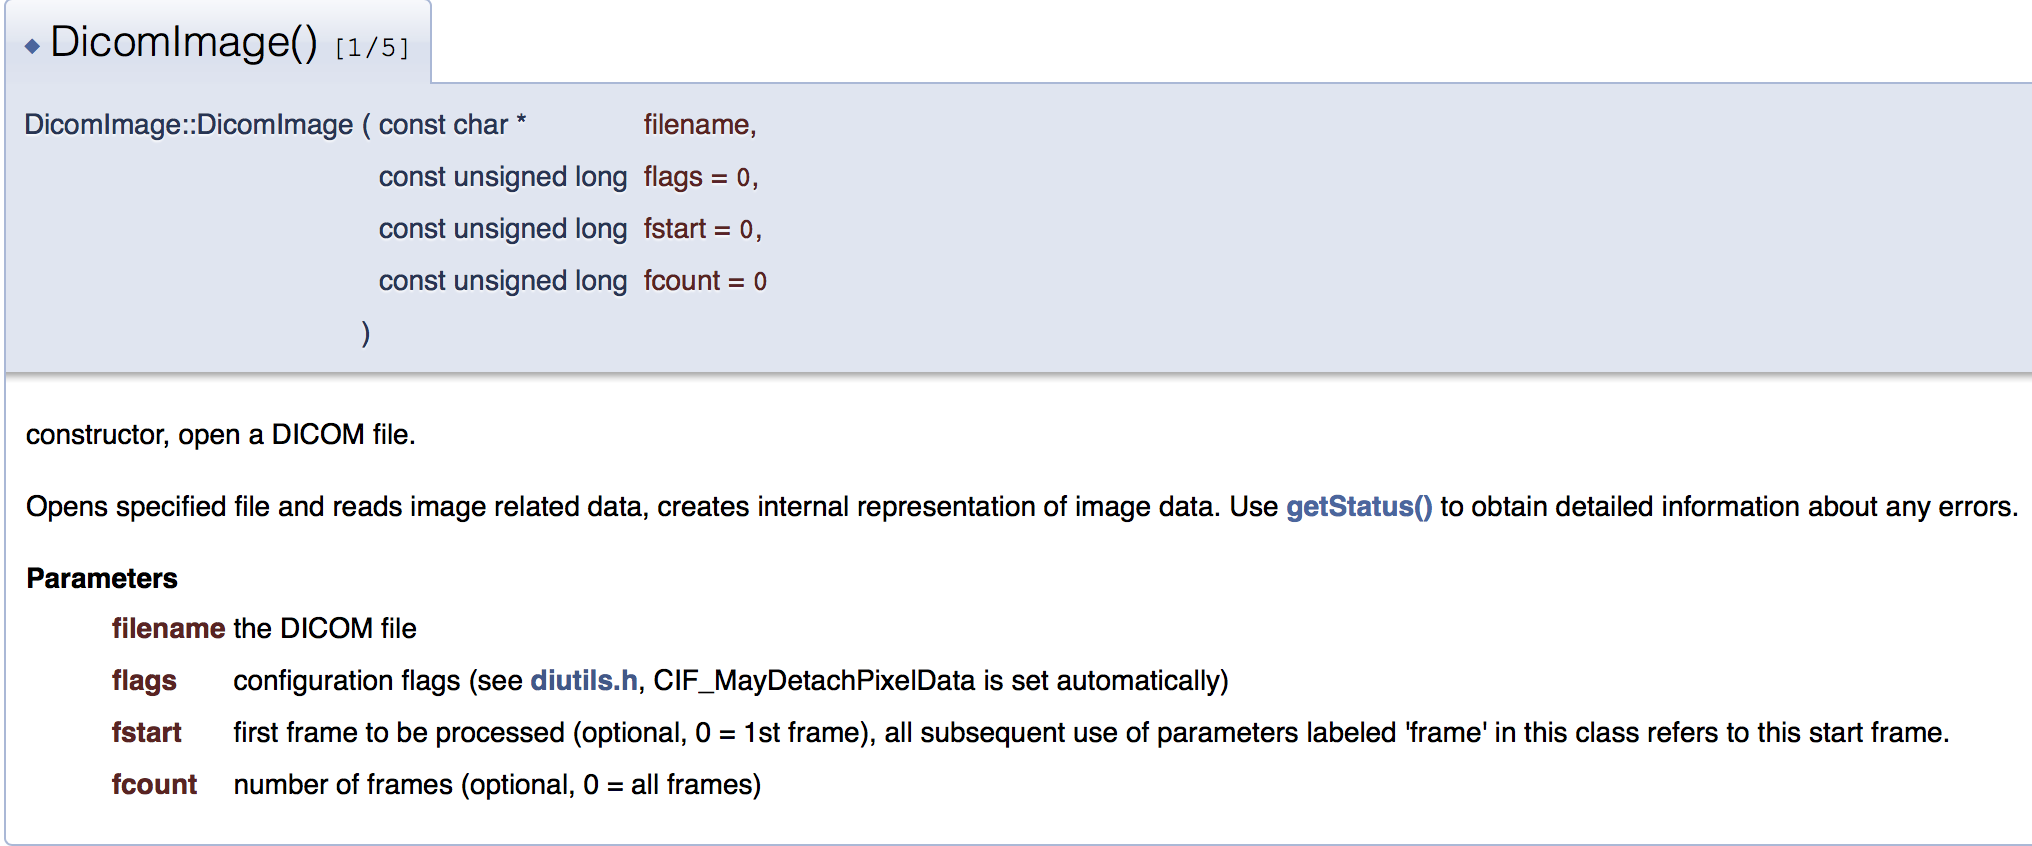
\includegraphics[width = 0.95\hsize]{./figures/DicomImageConstructor}
\caption{DicomImage Class Constructor}
\end{figure}


\begin{figure}[ht]
\centering
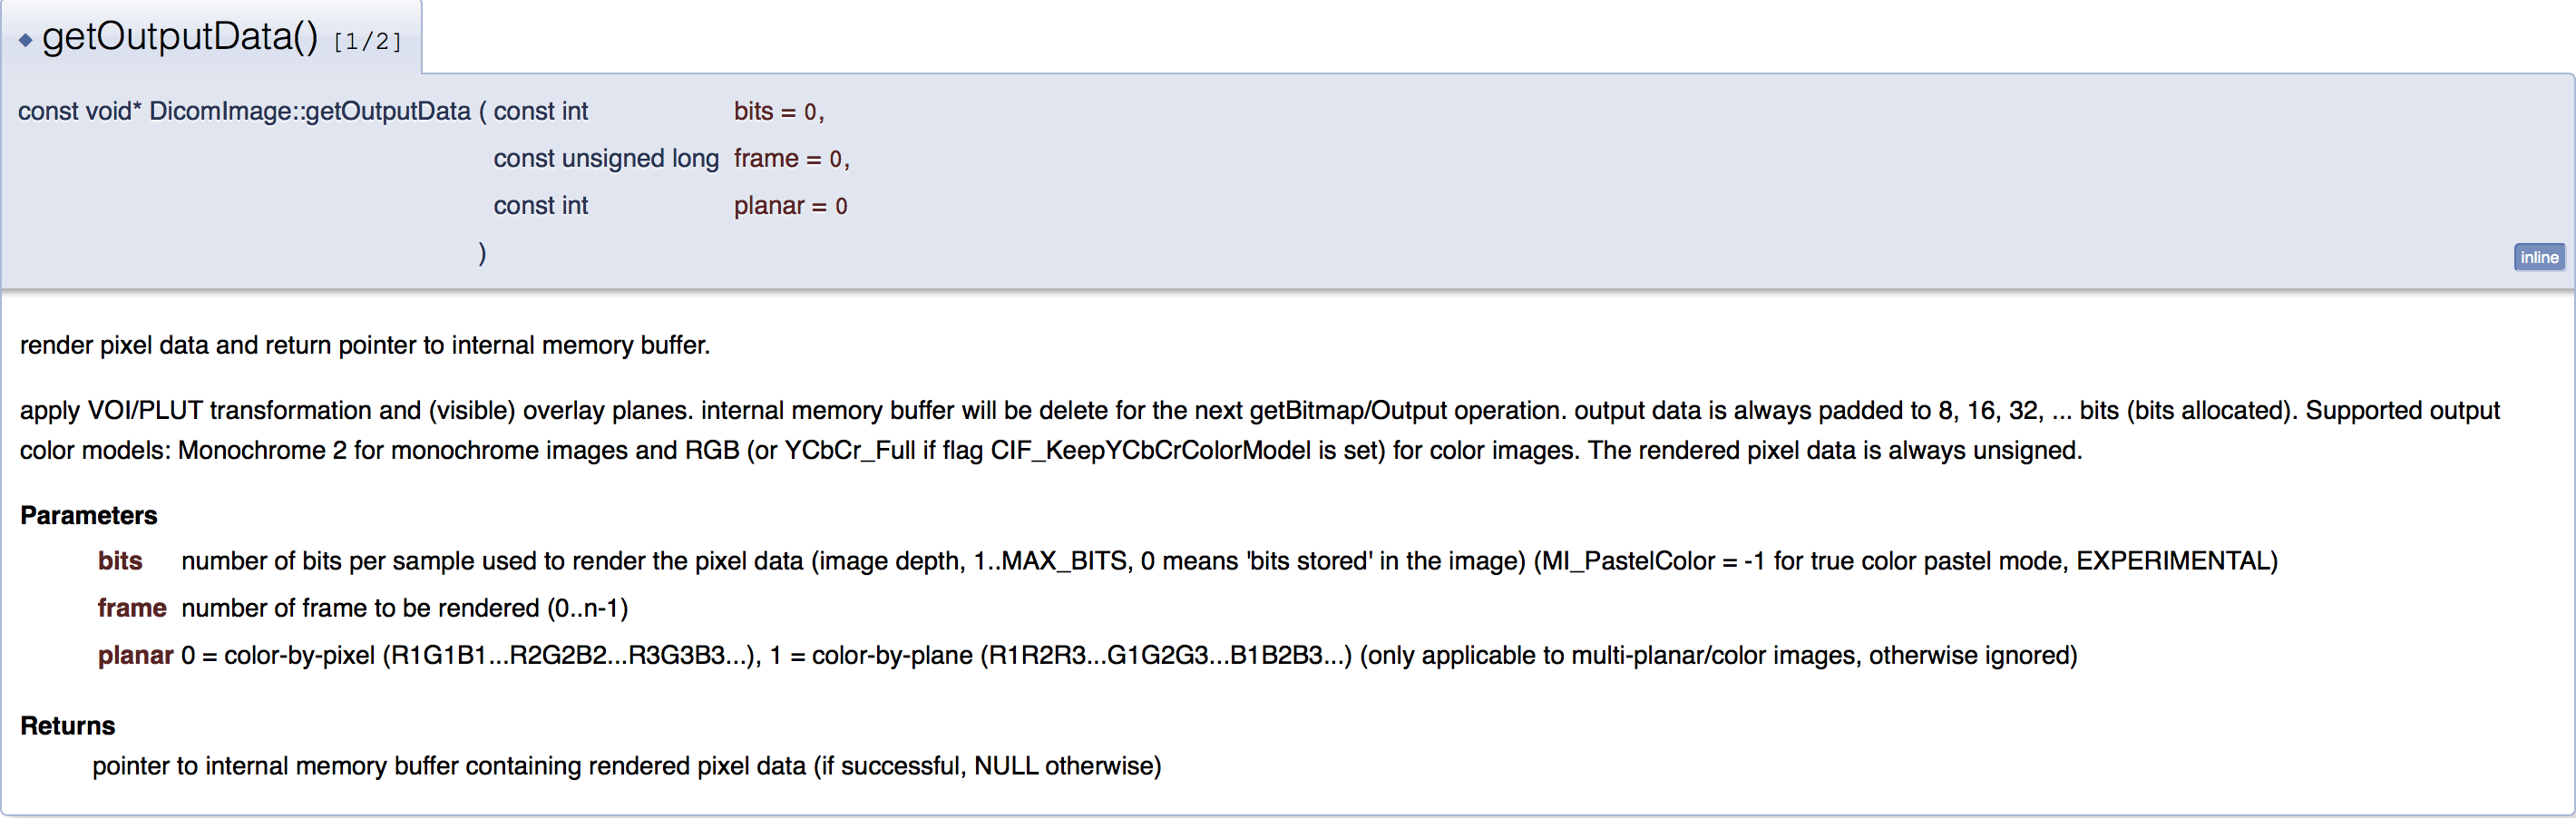
\includegraphics[width = 0.95\hsize]{./figures/getOutputData}
\caption{DicomImage getOutputData Function Definition}
\end{figure}

\clearpage
\subsection {Appendix 8 - Qt: Relevant classes and functions declarations}
\begin{figure}[ht]
\centering
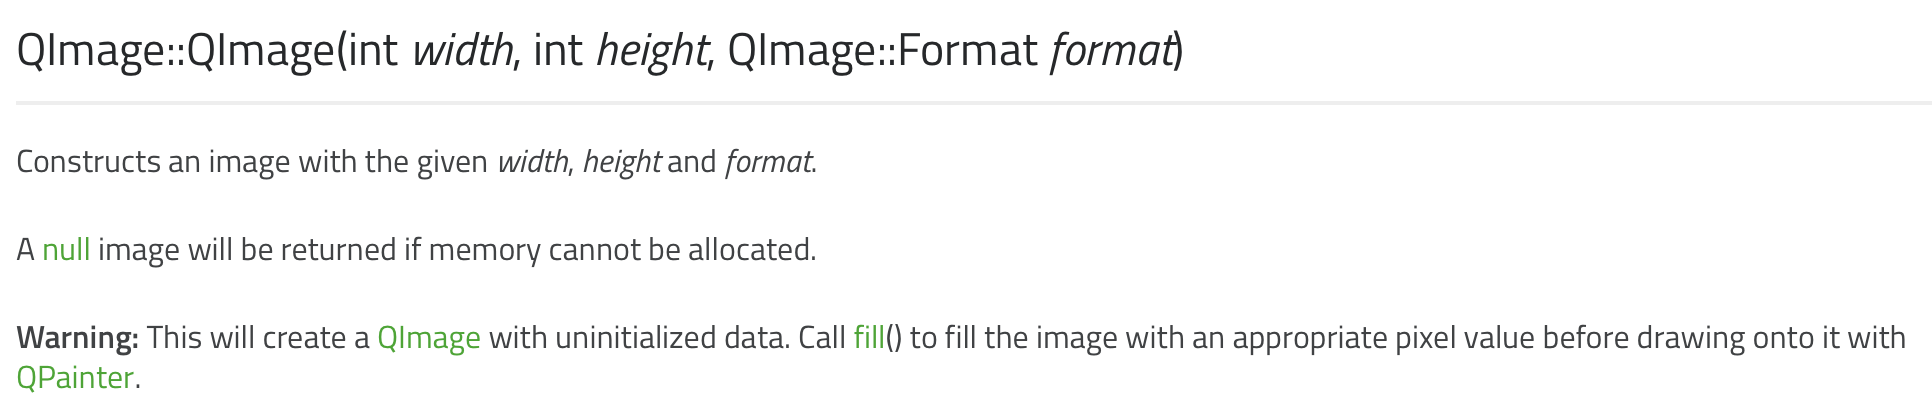
\includegraphics[width = 0.95\hsize]{./figures/QImage}
\caption{QImage contructor}
\end{figure}


\begin{figure}[ht]
\centering
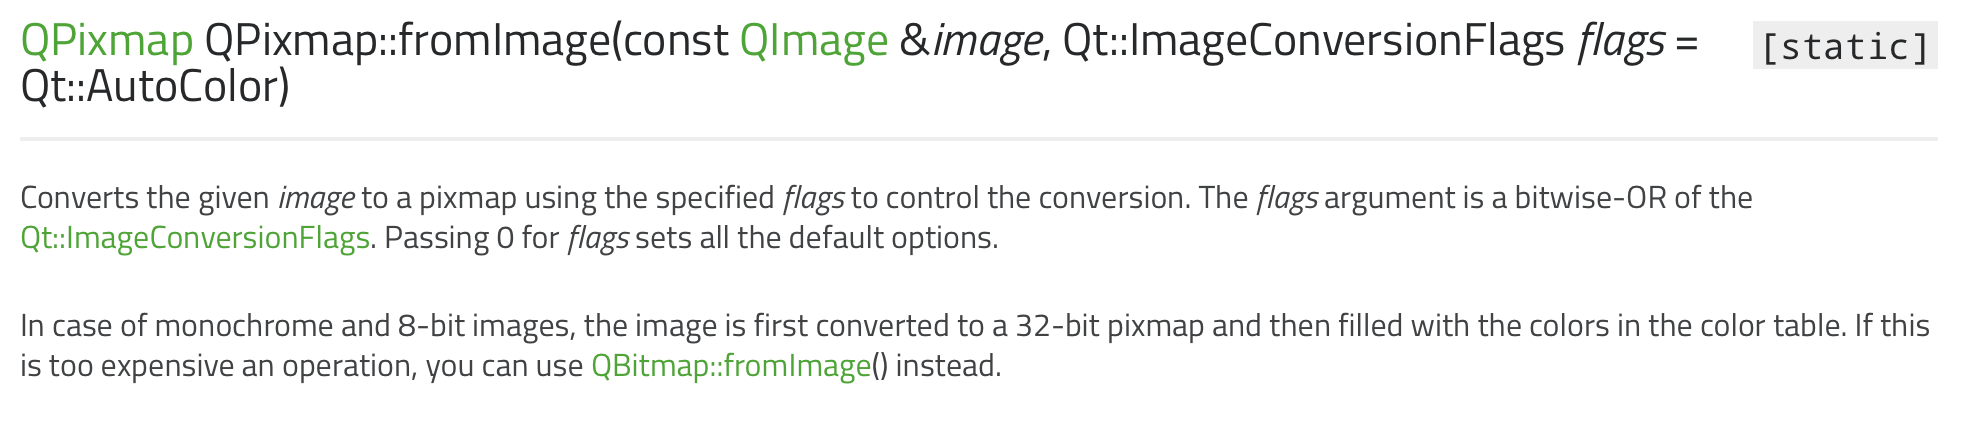
\includegraphics[width = 0.95\hsize]{./figures/QPixmap}
\caption{QPixmap static function}
\end{figure}

\clearpage
\subsection {Appendix 9 - Disclaimer}
\begin{figure}[ht]
\centering
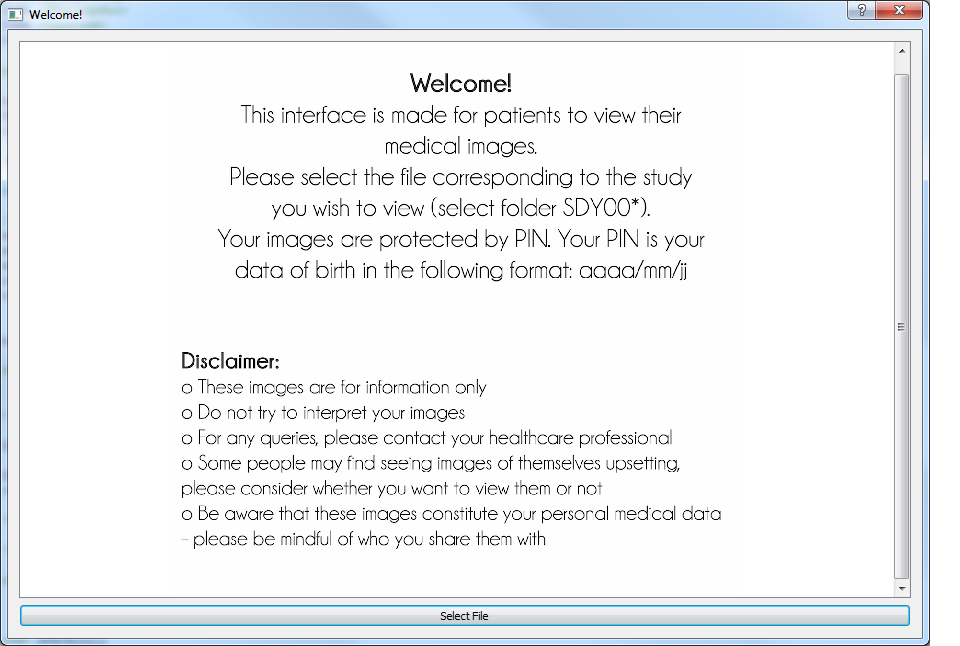
\includegraphics[width = 0.95\hsize]{./figures/screenshot/WelcomePage}
\caption{Welcome Window and Disclaimer}
\end{figure}

\clearpage
\subsection {Appendix 10 - Pin Access}
\begin{figure}[ht]
\centering
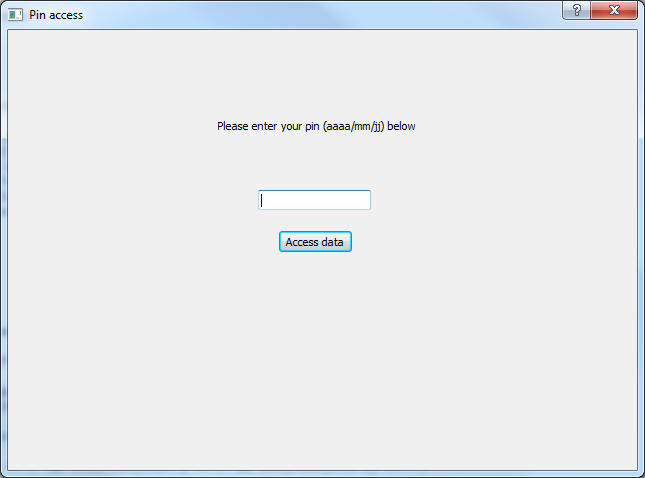
\includegraphics[width = 0.68\hsize]{./figures/screenshot/PinAccess1}
\caption{PIN Access Window }
\end{figure}
	

\begin{figure}[ht]
\centering
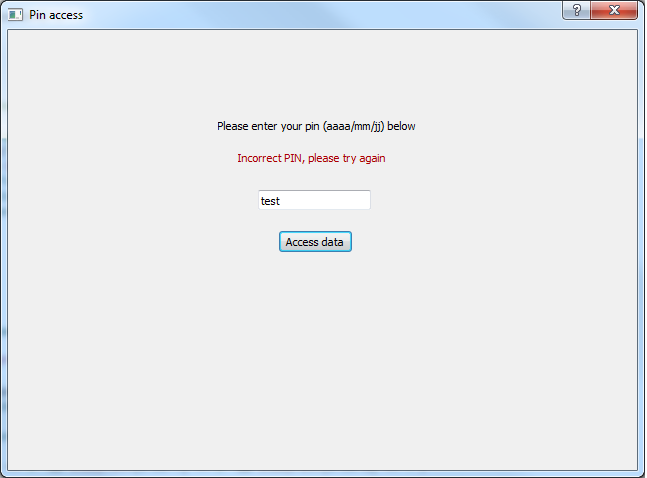
\includegraphics[width = 0.68\hsize]{./figures/screenshot/PinAccess2}
\caption{PIN Access Window in case of wrong provided PIN}
\end{figure}

\clearpage
\subsection {Appendix 11 - Main Window Overview}
\begin{figure}[ht]
\centering
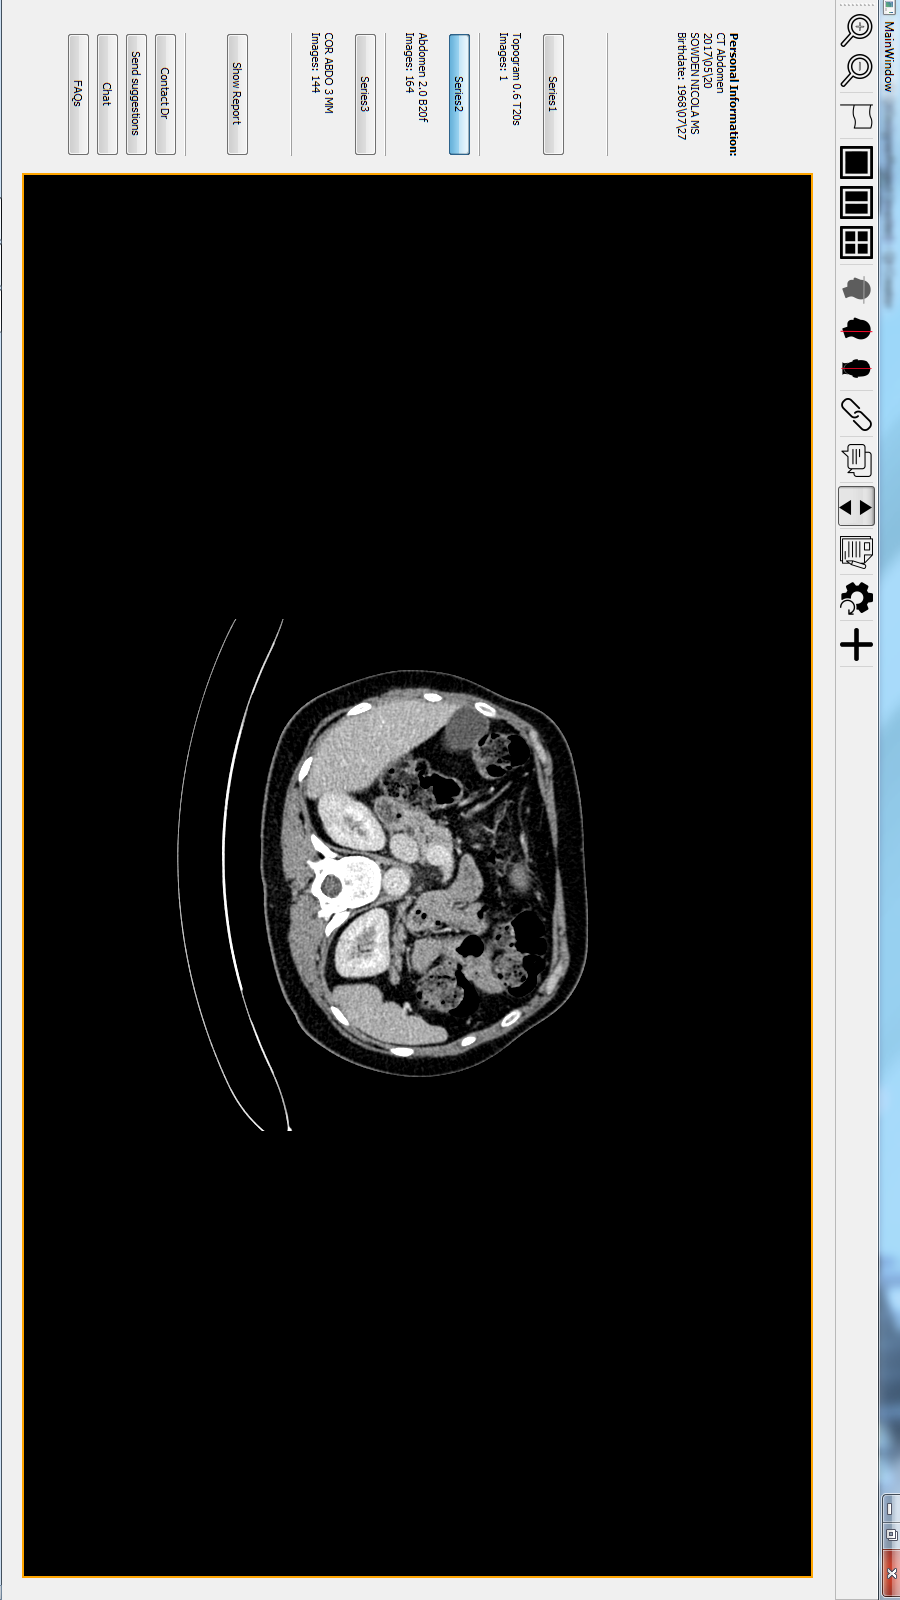
\includegraphics[width = 0.80\hsize]{./figures/screenshot/FirstPage}
\caption{Main Window Displaying CT Abdomen}
\end{figure}

\clearpage
\subsection {Appendix 12 - Reports Window}
\begin{figure}[ht]
\centering
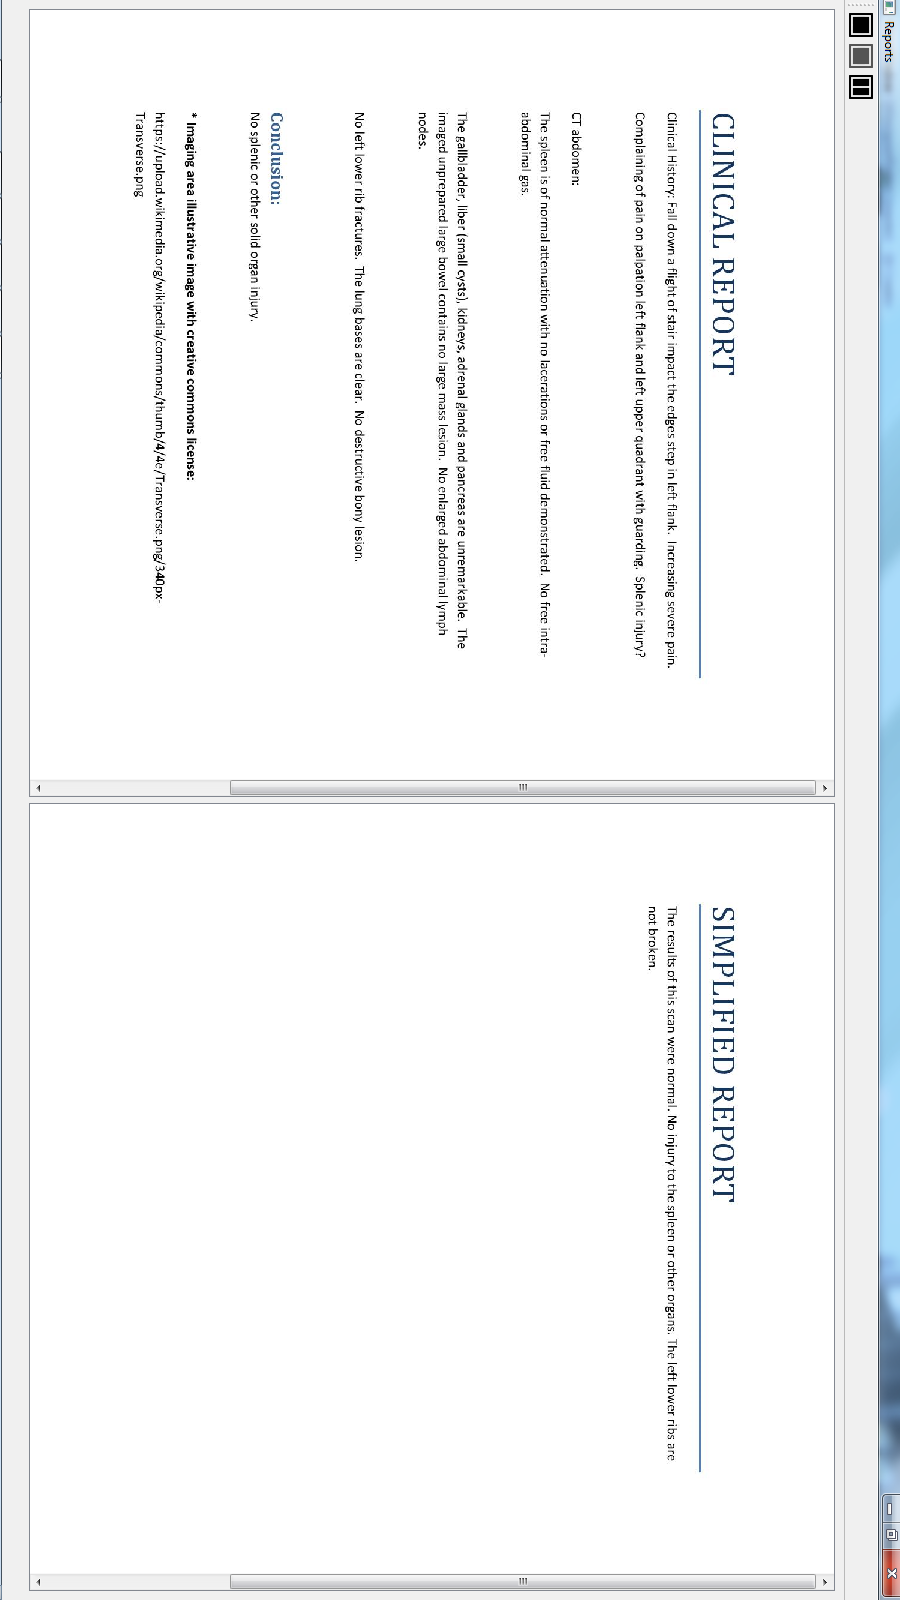
\includegraphics[width = 0.71\hsize]{./figures/screenshot/ReportWindow}
\caption{Overview of the Reports Window}
\end{figure}

%% bibliography
\printbibliography


\end{document}
